%% Modelo UNISINOS para Trabalhos de Conclusão de Curso (TCCs) baseado no abtex2-modelo-trabalho-academico.tex, v-1.9.5 laurocesar Copyright 2012-2015 by abnTeX2 group at http://www.abntex.net.br/ 
% ----------------------------------------------
% abnTeX2: Modelo de Trabalho Academico (tese de doutorado, dissertacao de mestrado e trabalhos monograficos em geral) em conformidade com ABNT NBR 14724:2011: Informacao e documentacao - Trabalhos academicos - Apresentacao
% ----------------------------------------------
% ==============================================
% ||||||||||||||||||||||||||||||||||||||||||||||
% ----------------------------------------------
\documentclass[
	% -- opções da classe memoir --
	12pt,				% tamanho da fonte
	openright,			% capítulos começam em pág ímpar (insere página vazia caso preciso)
	oneside,			% para impressão em verso e anverso. twoside Oposto a oneside
	a4paper,			% tamanho do papel. 
	% -- opções da classe abntex2 --
	chapter=TITLE,		% títulos de capítulos convertidos em letras maiúsculas
	%section=TITLE,		% títulos de seções convertidos em letras maiúsculas
	%subsection=TITLE,	% títulos de subseções convertidos em letras maiúsculas
	%subsubsection=TITLE,% títulos de subsubseções convertidos em letras maiúsculas
	% -- opções do pacote babel --
	english,			% idioma adicional para hifenização
%	french,				% idioma adicional para hifenização
%	spanish,			% idioma adicional para hifenização
	brazil				% o último idioma é o principal do documento
	]{abntex2} 
% ----------------------------------------------
% Pacotes de fontes... 
% ----------------------------------------------
\renewcommand{\ABNTEXchapterfont}{\fontfamily{ptm}\fontseries{sbc}\selectfont}
% \usepackage{lmodern}	% Usa a fonte Latin Modern
% \usepackage{fourier}	% Adobe utopia
% \usepackage{times}	% Usa a fonte Times, mas não muito boa
% \usepackage{palatino}	% Usa a fonte Palatino
% \usepackage{mathpazo}	% Usa a fonte Adobe Palatino

% \usepackage[scaled=.92]{helvet} % Usa a fonte Helvetica
% % Descomente a linha abaixo junto se for utilizar a fonte helvet
% \renewcommand{\familydefault}{\sfdefault}
\usepackage{mathptmx}
%\usepackage{tgtermes}
% Para entradas de capítulo com Times Bold usando um dos 2 pacotes acima
% \renewcommand{\ABNTEXchapterfont}{\rmfamily\bfseries}
% ----------------------------------------------
% Configuração das fontes
% ----------------------------------------------
% Algumas configurações de fontes para capitulos e seções tanto no texto quanto no sumário
\renewcommand{\ABNTEXchapterfont}{\bfseries}
\renewcommand{\ABNTEXchapterfontsize}{\Large}
\renewcommand{\ABNTEXpartfont}{\ABNTEXchapterfont}
\renewcommand{\ABNTEXpartfontsize}{\ABNTEXchapterfontsize}
\renewcommand{\cftpartfont}{\normalfont\bfseries}
\renewcommand{\ABNTEXsectionfont}{\bfseries}
\renewcommand{\ABNTEXsectionfontsize}{\large}
\renewcommand{\ABNTEXsubsectionfont}{\normalfont}
\renewcommand{\ABNTEXsubsectionfontsize}{\normalsize}
\renewcommand{\cftsubsectionfont}{\normalfont}
\renewcommand{\ABNTEXsubsubsectionfont}{\slshape}
\renewcommand{\cftsubsubsectionfont}{\normalfont\slshape}
\renewcommand{\ABNTEXsubsubsubsectionfont}{\bfseries}
% Para configurar mais níveis configure conforme utilizado acima e comente as duas linhas abaixo
\settocdepth{subsubsection} % configura sumário para apresentar subseções até o quarto nível
\setsecnumdepth{subsubsection} % configura para numerar subseções até o quarto nível. Subseções de quinto nível não conterão numeração.
\addto\captionsbrazil{\renewcommand{\listfigurename}{Lista de figuras}} % Altera nome da lista de ilustrações para lista de figuras
% \addto{\captionsbrazil}{\renewcommand{\bibname}{Referências Bibliográficas}}
% ----------------------------------------------
% Equações com numeração sequencial
% ----------------------------------------------
\usepackage{chngcntr}
\counterwithout{equation}{chapter}
% ----------------------------------------------
% Pacotes básicos 
% ----------------------------------------------
\usepackage[T1]{fontenc}	% Selecao de codigos de fonte.
\usepackage[utf8]{inputenc}	% Codificacao do documento (conversão automática dos acentos)
\usepackage{lastpage}		% Usado pela Ficha catalográfica
\usepackage{indentfirst} 	% Indenta o primeiro parágrafo de cada seção.
\usepackage{color, colortbl}% Controle das cores
\usepackage{float}
\usepackage{graphicx}		% Inclusão de gráficos
\usepackage{microtype} 		% para melhorias de justificação
\usepackage{array}
%\usepackage{gensymb}       % Símbolos
\usepackage{amsmath} 	%--------------------------%
\usepackage{hyperref} 	%--------------------------%
\usepackage{bibentry} 	% para inserir refs. bib. no meio do texto
% ----------------------------------------------
% Pacotes adicionais
% ----------------------------------------------
\usepackage{lipsum}	% para geração de dummy text
\usepackage[colorinlistoftodos, english]{todonotes}
  % exemplos de uso: 
  %\todo[inline, color=red!80]{texto}
\usepackage{verbatim}
\usepackage{soulutf8}
  % exemplos de uso: 
  %\hl{highlight} ou \st{strikeout} ou \ul{underline}
\usepackage{tabularx}
\usepackage{multirow}
%\usepackage{subfig}
\usepackage{pdfpages}
\usepackage{pgfplots}
  \pgfplotsset{compat=1.12}
% Para desenho de circuitos
\usepackage{tikz}
\usepackage[american]{circuitikz}
\usepackage{siunitx}
\sisetup{locale = FR}

% ---
% Formatação de código-fonte
% ---
\usepackage{listings}

% Altera o nome padrão do rótulo usado no comando \autoref{}
\renewcommand{\lstlistingname}{Código}

% Altera o rótulo a ser usando no elemento pré-textual "Lista de código"
\renewcommand{\lstlistlistingname}{Lista de códigos}

% Configura a ``Lista de Códigos'' conforme as regras da ABNT (para abnTeX2)
\begingroup\makeatletter
\let\newcounter\@gobble\let\setcounter\@gobbletwo
  \globaldefs\@ne \let\c@loldepth\@ne
  \newlistof{listings}{lol}{\lstlistlistingname}
  \newlistentry{lstlisting}{lol}{0}
\endgroup

\renewcommand{\cftlstlistingaftersnum}{\hfill--\hfill}

\let\oldlstlistoflistings\lstlistoflistings
\renewcommand{\lstlistoflistings}{%
   \begingroup%
   \let\oldnumberline\numberline%
   \renewcommand{\numberline}{\lstlistingname\space\oldnumberline}%
   \oldlstlistoflistings%
   \endgroup}



\usepackage{color}
\definecolor{dkgreen}{rgb}{0,0.6,0}
\definecolor{gray}{rgb}{0.5,0.5,0.5}
\definecolor{mauve}{rgb}{0.58,0,0.82}
\lstset{frame=tb,
  language=C,
  aboveskip=3mm,
  belowskip=3mm,
  showstringspaces=false,
  columns=flexible,
  basicstyle={\small\ttfamily},
  numbers=left,
  numberstyle=\tiny\color{gray},
  keywordstyle=\color{blue},
  commentstyle=\color{dkgreen},
  stringstyle=\color{mauve},
  breaklines=true,
  breakatwhitespace=true,
  tabsize=3
}     
% ----------------------------------------------
% Pacotes de citações
% ----------------------------------------------
\usepackage[brazilian,hyperpageref]{backref}	 % Paginas com as citações na bibl
\usepackage[alf, abnt-etal-text=it]{abntex2cite} % Citações padrão ABNT
% ==============================================
% CONFIGURAÇÕES DE PACOTES
% ==============================================
% ----------------------------------------------
% Configurações do pacote backref
% Usado sem a opção hyperpageref de backref
% ----------------------------------------------
\renewcommand{\backrefpagesname}{Citado na(s) página(s):~}
% Texto padrão antes do número das páginas
\renewcommand{\backref}{}
% Define os textos da citação
\renewcommand*{\backrefalt}[4]{
	\ifcase #1 %
		Nenhuma citação no texto.%
	\or
		Citado na página #2.%
	\else
		Citado #1 vezes nas páginas #2.%
	\fi}%
% ||||||||||||||||||||||||||||||||||||||||||||||
% Informações de dados para CAPA e FOLHA DE ROSTO
% ||||||||||||||||||||||||||||||||||||||||||||||
\titulo{DETECÇÃO E DIAGNÓSTICO AUTOMÁTICO DE FALHAS EM MOTORES ELÉTRICOS DE INDUÇÃO VIA ANÁLISE DE ASSINATURAS NA CORRENTE ELÉTRICA E VIBRAÇÃO}
\autor{GUILHERME ANGELO PIAIA}
\local{São Leopoldo, RS}
\data{2021}
\orientador{Prof. Dr. Rodrigo Marques de Figueiredo} 
%Nome completo do professor com sua titulação (Esp. ou MS. ou Dr.)
%\coorientador{Prof. Dr. }
\instituicao{%
  UNIVERSIDADE DO VALE DO RIO DOS SINOS - UNISINOS
  \par
  UNIDADE ACADÊMICA DE PESQUISA E PÓS-GRADUAÇÃO
  \par
  PROGRAMA DE PÓS-GRADUAÇÃO EM ENGENHARIA ELÉTRICA
  \par
  NÍVEL MESTRADO PROFISSIONAL}

\tipotrabalho{Dissertação (Mestrado)}
% O preambulo deve conter o tipo do trabalho, o objetivo, o nome da instituição e a área de concentração 
% Verifique a nomenclatura utilizada: Graduado, Bacharel ou Licenciado junto à Coordenação do seu Curso.
\preambulo{Dissertação apresentada como requisito parcial para obtenção do título de Mestre em Engenharia Elétrica,
 pelo Programa de Pós-Graduação em Engenharia Elétrica da Universidade do Vale do Rio dos Sinos - UNISINOS.}
% ----------------------------------------------
% Configurações de aparência do PDF final
% ----------------------------------------------
% alterando o aspecto da cor azul
\definecolor{blue}{RGB}{41,5,195}
% alterando o aspecto da cor cinza
\definecolor{gray}{RGB}{50,50,50}
% informações do PDF
\makeatletter
\hypersetup{
    %pagebackref=true,
    pdftitle={\imprimirtitulo}, 
    pdfauthor={\imprimirautor},
    pdfsubject={\imprimirpreambulo},
	pdfcreator={LaTeX - abnTeX2 - Overleaf},
	pdfkeywords={abnt}{latex}{abntex2}{trabalho acadêmico}{unisinos}{engenharia de controle e automação}{tcc},
    colorlinks=true, % false: boxed links; true: colored links
    linkcolor=black, % color of internal links
    citecolor=black, % color of links to bibliography
    filecolor=blue,  % color of file links
    urlcolor=gray,
    bookmarksdepth=4
}
\makeatother
% ----------------------------------------------
% Espaçamentos entre linhas e parágrafos 
% ----------------------------------------------
% O tamanho do parágrafo é dado por:
\setlength{\parindent}{1.3cm}
% Controle do espaçamento entre um parágrafo e outro:
\setlength{\parskip}{0.2cm}  % tente também \onelineskip
% ----------------------------------------------
% compila o indice
% ----------------------------------------------
\makeindex

% ----------------------------------------------
% Pacotes extras
% ----------------------------------------------
%\newcommand*\cuk{\´{C}}
 \addto{\captionsbrazil}{\renewcommand{\bibname}{Referências Bibliográficas}}
\newcommand{\cuk}{\'Cuk}
\usepackage{booktabs}
\usepackage{adjustbox}
\usepackage{graphicx}
\usepackage{placeins}
\usepackage{longtable}
\usepackage{caption}
\usepackage{subcaption}
\usepackage{graphicx}
% ----------------------------------------------
% ||||||||||||||||||||||||||||||||||||||||||||||
% Início do documento
% ||||||||||||||||||||||||||||||||||||||||||||||
\begin{document}
% Seleciona o idioma do documento (conforme pacotes do babel)
%\selectlanguage{english}
\selectlanguage{brazil}
% Retira espaço extra obsoleto entre as frases.
\frenchspacing 
% Adiciona lista de correções no início do documento.
% Comentar a linha abaixo quando o trabalho for concluído
%\listoftodos
\newpage
% ==============================================
% ELEMENTOS PRÉ-TEXTUAIS\newcolumntype{C}[1]{>{\centering\arraybackslash}m{#1}<{}}
\newcolumntype{L}[1]{>{\raggedright\arraybackslash}m{#1}<{}}
\newcolumntype{R}[1]{>{\raggedleft\arraybackslash}m{#1}<{}}
% ==============================================
\pretextual
% ----------------------------------------------
% Capa
% ----------------------------------------------
%\imprimircapa
% Capa personalizada sem o uso de \imprimircapa
\begin{capa}

% \renewcommand{\arraystretch}{0.9}%
% \noindent\begin{tabularx}{\textwidth}{l @{\extracolsep{\fill}} >{\small} r}
% \multirow{3}{*}{\includegraphics[width = 2.9cm]{images/unisinos_logo_bw.png}} 
%  & \MakeUppercase{{Universidade do Vale do Rio dos Sinos}} \\ 
%  & Escola Politécnica \\
%  & Programa de Pós-Graduação em Engenharia Elétrica \\
% \bottomrule
% \end{tabularx}
% \renewcommand{\arraystretch}{1}%
    \center
    \ABNTEXchapterfont\large{\imprimirinstituicao}
    \vfill
    %\vspace*{1cm}
	\MakeUppercase{
    \ABNTEXchapterfont\textsc{\imprimirautor}}
    \vfill
    \begin{center}
    \ABNTEXchapterfont\bfseries\Large\imprimirtitulo
    \end{center}
    \vfill
	\vspace*{5cm}
    \large\imprimirlocal \\
    \large\imprimirdata
    \vspace*{1cm}
\end{capa}
 
% ----------------------------------------------
% Folha de rosto (o * indica que haverá a ficha bibliográfica)
% ----------------------------------------------
% %\imprimirfolhaderosto*
% % folha de rosto personalizada
% \makeatletter
% \renewcommand{\folhaderostocontent}{
% \begin{center}
%   {\ABNTEXchapterfont\large\imprimirautor}
%   \vspace*{\fill}%\vspace*{\fill}
%   \begin{center}
%   \ABNTEXchapterfont\bfseries\Large\imprimirtitulo
%   \end{center}
%   \vspace*{\fill}
  
%   \abntex@ifnotempty{\imprimirpreambulo}{%
%     \hspace{.45\textwidth}
%     \begin{minipage}{.5\textwidth}
%     \SingleSpacing
%     \imprimirpreambulo
%     \end{minipage}%
%     \vspace*{\fill}
%   }%

%   \abntex@ifnotempty{\imprimirorientador}{%
%   \hspace{.45\textwidth}
%   \begin{minipage}{.5\textwidth}
% 	{\large\imprimirorientadorRotulo \\ 
%      \imprimirorientador
%      \par}%
%   \end{minipage}%
%   }%
  
%   \abntex@ifnotempty{\imprimircoorientador}{%
%   \hspace{.45\textwidth}
%   \begin{minipage}{.5\textwidth}
% 	{\large\imprimircoorientadorRotulo \\ 
%      \imprimircoorientador
%      \par}%
%   \end{minipage}%
%   }%
  
%   \vspace*{\fill}

% %{\abntex@ifnotempty{\imprimirinstituicao}{\imprimirinstituicao\vspace*{\fill}}}
%   {\large\imprimirlocal}
%   \par
%   {\large\imprimirdata}
%   \vspace*{1cm}
%   \end{center}
%   }
% \makeatother
% % Folha de rosto (o * indica que haverá a ficha bibliográfica)
% \imprimirfolhaderosto



% ----------------------------------------------
% Folha de rosto (o * indica que haverá a ficha bibliográfica)
% ----------------------------------------------
%\imprimirfolhaderosto*
% folha de rosto personalizada
\makeatletter
\renewcommand{\folhaderostocontent}{
\begin{center}
  {\ABNTEXchapterfont\large\imprimirautor}
  \vspace*{\fill}%\vspace*{\fill}
  \begin{center}
  \ABNTEXchapterfont\bfseries\Large\imprimirtitulo
  \end{center}
  \vspace*{\fill}
  
  \abntex@ifnotempty{\imprimirpreambulo}{%
    \hspace{.45\textwidth}
    \begin{minipage}{.5\textwidth}
    \SingleSpacing
    \imprimirpreambulo
    \end{minipage}%
    \vspace*{\fill}
  }%

  \abntex@ifnotempty{\imprimirorientador}{%
  \hspace{.45\textwidth}
  \begin{minipage}{.5\textwidth}
	{\large\imprimirorientadorRotulo \\ 
     \imprimirorientador
     \par}%
  \end{minipage}%
  }%
  
  \abntex@ifnotempty{\imprimircoorientador}{%
  \hspace{.45\textwidth}
  \begin{minipage}{.5\textwidth}
	{\large\imprimircoorientadorRotulo \\ 
     \imprimircoorientador
     \par}%
  \end{minipage}%
  }%
  
  \vspace*{\fill}

%{\abntex@ifnotempty{\imprimirinstituicao}{\imprimirinstituicao\vspace*{\fill}}}
  {\large\imprimirlocal}
  \par
  {\large\imprimirdata}
  \vspace*{1cm}
  \end{center}
  }
\makeatother


% Folha de rosto (o * indica que haverá a ficha bibliográfica)
\makeatletter
\renewcommand{\folhaderostocontent}{
\begin{center}
  {\ABNTEXchapterfont\large\imprimirautor}
  \vspace*{\fill}%\vspace*{\fill}
  \begin{center}
  \ABNTEXchapterfont\bfseries\Large\imprimirtitulo
  \end{center}
  \vspace*{\fill}
  
  \abntex@ifnotempty{\imprimirpreambulo}{%
    \hspace{.45\textwidth}
    \begin{minipage}{.5\textwidth}
    \SingleSpacing
    \imprimirpreambulo
    \end{minipage}%
    \vspace*{\fill}
  }%

  \abntex@ifnotempty{\imprimirorientador}{%
  \hspace{.45\textwidth}
  \begin{minipage}{.5\textwidth}
  {\large\imprimirorientadorRotulo \\ 
     \imprimirorientador
     \par}%
  \end{minipage}%
  }%
  
  \abntex@ifnotempty{\imprimircoorientador}{%
  \hspace{.45\textwidth}
  \begin{minipage}{.5\textwidth}
  {\large\imprimircoorientadorRotulo \\ 
     \imprimircoorientador
     \par}%
  \end{minipage}%
  }%
  
  \vspace*{\fill}
%{\abntex@ifnotempty{\imprimirinstituicao}{\imprimirinstituicao\vspace*{\fill}}}
  {\large\imprimirlocal}
  \par
  {\large\imprimirdata}
  \vspace*{1cm}
  \end{center}
  }
\makeatother
% Folha de rosto (o * indica que haverá a ficha bibliográfica)
 \imprimirfolhaderosto*

% ----------------------------------------------
% Inserir a ficha bibliografica catalográfica
% ----------------------------------------------
% % % Isto é um exemplo de Ficha Catalográfica, ou ``Dados internacionais de catalogação-na-publicação''. Você pode utilizar este modelo como referência. Porém, provavelmente a biblioteca da sua universidade lhe fornecerá um PDF com a ficha catalográfica definitiva após a defesa do trabalho. Quando estiver com o documento, salve-o como PDF no diretório do seu projeto e substitua todo o conteúdo de implementação deste arquivo pelo comando abaixo:

%%\begin{fichacatalografica}
  %%  \includepdf{fig_ficha_catalografica.pdf}
%%\end{fichacatalografica}

\begin{fichacatalografica}
	\sffamily
	\vspace*{\fill}					% Posição vertical
  	\begin{center}					% Minipage Centralizado
	\fbox{
    \begin{minipage}[t]{1,5cm} 
    \vspace{0.5cm} 
    D383m %Algum número que o bibliotecario ira gerar
    \end{minipage}
    
    \begin{minipage}[t]{11cm}	% Largura
	\small
    \vspace{0.5cm}
	%\imprimirautor		% ATENCAO - SUBSTITUIR POR %Sobrenome, Nome do autor
    Cavalheiro, Guilherme Eduardo
	
	\hspace{0.5cm} 
    \imprimirtitulo  / \imprimirautor. -- \imprimirdata.
	
	\hspace{0.5cm} 
    \pageref{LastPage} p. : il. (algumas color.) ; 30 cm.\\
	
    \hspace{0.5cm}
	\imprimirtipotrabalho~--~Universidade do Vale do Rio dos Sinos, Curso de Engenharia Elétrica, São Leopoldo, RS, \imprimirdata. \hfill 
    
    \hspace{0.5cm}
    \imprimirorientadorRotulo~\imprimirorientador ;
    \imprimircoorientadorRotulo~\imprimircoorientador\\
	
	\hspace{0.5cm}
		1. Palavra-chave1
		2. Palavra-chave1
		3. Palavra-chave1
        I. Título \\
		%I. \imprimirtitulo \\
        %II. \imprimirorientador \\
    
	\hspace{8.75cm} CDU 621.3 %algum outro numero
	
    \end{minipage}}
    
    \hspace{0.5cm}
    Dados Internacionais de Catalogação na Publicação (CIP) \\  	(Bibliotecário: Nome Sobrenome – CRB 10/1298)
	
    \end{center}
\end{fichacatalografica}
 
% ----------------------------------------------
% Inserir errata
% ----------------------------------------------
%% \begin{errata}
% Elemento opcional da \citeonline[4.2.1.2]{NBR14724:2011}. Exemplo:

% \vspace{\onelineskip}

% FERRIGNO, C. R. A. \textbf{Tratamento de neoplasias ósseas apendiculares com
% reimplantação de enxerto ósseo autólogo autoclavado associado ao plasma
% rico em plaquetas}: estudo crítico na cirurgia de preservação de membro em
% cães. 2011. 128 f. Tese (Livre-Docência) - Faculdade de Medicina Veterinária e
% Zootecnia, Universidade de São Paulo, São Paulo, 2011.

% \begin{table}[htb]
% \center
% \footnotesize
% \begin{tabular}{|p{1.4cm}|p{1cm}|p{3cm}|p{3cm}|}
%   \hline
%    \textbf{Folha} & \textbf{Linha}  & \textbf{Onde se lê}  & \textbf{Leia-se}  \\
%     \hline
%     1 & 10 & auto-conclavo & autoconclavo\\
%    \hline
% \end{tabular}
% \end{table}

% \end{errata} 
% ----------------------------------------------
% Folha de aprovação
% ----------------------------------------------
% % ----------------------------------------------
% Inserir folha de aprovação
% ----------------------------------------------

% Isto é um exemplo de Folha de aprovação, elemento obrigatório da NBR
% 14724/2011 (seção 4.2.1.3). Você pode utilizar este modelo até a aprovação
% do trabalho. Após isso, substitua todo o conteúdo deste arquivo por uma
% imagem da página assinada pela banca com o comando abaixo:

% \includepdf{folhadeaprovacao_final.pdf}

\begin{folhadeaprovacao}
% Gerada conforme instrucoes do PPGEE
  \begin{center}
  {\ABNTEXchapterfont\large\imprimirautor}

  \vspace*{\fill}\vspace*{\fill}
    \begin{center}
    	\ABNTEXchapterfont\bfseries\Large\imprimirtitulo
    \end{center}
  \vspace*{\fill}

  \hspace{.45\textwidth}
    \begin{minipage}{.5\textwidth}
    	\imprimirpreambulo 
    \end{minipage}%

  \vspace*{\fill}
    \begin{flushleft}
  	  Aprovado em x de y de 2016. \\
    \end{flushleft}
  \vspace*{\fill}
    BANCA EXAMINADORA:% \imprimirlocal, \today :
  \end{center}
   
   %\assinatura{\textbf{\imprimirorientador} \\ Orientador}
   %\assinatura{\textbf{\imprimircoorientador} \\ Coorientador} 
   \assinatura{Prof. Dr. Nome Sobrenome -- UNISINOS \\ Avaliador}
   \assinatura{Prof. Dr. Nome Sobrenome -- UNISINOS \\ Avaliador}
   \assinatura{Prof. Dr. Nome Sobrenome -- UNISINOS \\ Avaliador Externo}
    \vspace*{\fill} \vspace*{\fill}
    \hspace{.4\textwidth}
    \begin{minipage}{.5\textwidth}
    	\imprimirorientador~\\(Orientador) \\
		%\imprimircoorientador~(Coorientador)
    \end{minipage}%
    
    \vspace*{\fill}
    \begin{flushleft}
    	Visto e permitida a impressão\\
        \imprimirlocal
    \end{flushleft}
    
    \vspace*{\fill}
    \hspace{.4\textwidth}
    \begin{minipage}{.5\textwidth}
    	Prof. Dr. Lúcio Rene Prade \\
        Coordenador do Curso de Engenharia Elétrica
    \end{minipage}%
%    \begin{center}
%     \vspace*{0.5cm}
%       {\large\imprimirlocal}
%       \par
%       {\large\imprimirdata}
%       \vspace*{1cm}
%   \end{center}
  
\end{folhadeaprovacao} 
% ----------------------------------------------
% Dedicatória
% ----------------------------------------------
\begin{dedicatoria}
   \vspace*{\fill}
   \centering
   \noindent
    \textit{Este trabalho é dedicado aos meus pais que, com muito carinho e apoio,\\
    não mediram esforços para que eu chegasse até esta etapa de minha vida.} 
   \vspace*{\fill}
\end{dedicatoria} 
% ----------------------------------------------
% Agradecimentos
% ----------------------------------------------
\begin{agradecimentos}
	Aos familiares, namorada, amigos e professores, pelo incentivo e pelo apoio constante nesta etapa
	de minha vida.
\end{agradecimentos} 
% ----------------------------------------------
% Epígrafe
% ----------------------------------------------
\begin{epigrafe}
    \vspace*{\fill}
	\begin{flushright}
		\textit{``Science can amuse and fascinate us all, but it is engineering that changes the world" \\
        (Isaac Asimov)}
	\end{flushright}
\end{epigrafe} 
% ||||||||||||||||||||||||||||||||||||||||||||||
% RESUMOS
% ||||||||||||||||||||||||||||||||||||||||||||||
% ----------------------------------------------
% resumo em português
% ----------------------------------------------
\setlength{\absparsep}{18pt} % ajusta o espaçamento dos parágrafos do resumo
\begin{resumo}
    \lipsum[7]    
	\vspace{\onelineskip}
	\noindent 
	\textbf{Palavras-chaves}: latex. abntex. text editoration.
\end{resumo}

% ----------------------------------------------
% resumo em inglês
% ----------------------------------------------
\begin{resumo}[Abstract]
 \begin{otherlanguage*}{english}
   This is the english abstract.
   \lipsum[7]
   \vspace{\onelineskip}
 
   \noindent 
   \textbf{Keywords}: latex. abntex. text editoration.
 \end{otherlanguage*}
\end{resumo}
 
% ||||||||||||||||||||||||||||||||||||||||||||||
% Listas
% ||||||||||||||||||||||||||||||||||||||||||||||
% ----------------------------------------------
% inserir lista de ilustrações
% ----------------------------------------------
\pdfbookmark[0]{\listfigurename}{lof}
\listoffigures*
\cleardoublepage
% ----------------------------------------------
% inserir lista de tabelas
% ----------------------------------------------
\pdfbookmark[0]{\listtablename}{lot}
\listoftables*
\cleardoublepage
% ----------------------------------------------
% inserir lista de abreviaturas e siglas
% ----------------------------------------------
% Deve conter a relação alfabética das siglas utilizadas no texto, seguidas das palavras ou das expressões escritas por extenso.
\begin{siglas}
%   \item[ABNT] Associação Brasileira de Normas Técnicas
%   \item[NBR] Normas Brasileiras de Regulação
\item[PID] \textit{Proportionl, Integral and Derivative} (Proporcional, Integral e Derivativo)
\item[PI] \textit{Proportionl and Integral} (Proporcional e Integral)
\item[AD] \textit{Analógico-Digital}
\item[UNISINOS]  \textit{Universidade do Vale do Rio dos Sinos}
\item[URSS]  \textit{União das Repúblicas Socialistas Soviéticas}
\item[GPIO]  \textit{General Purpose Input/Output} (Entradas e Saídas de uso Geral)
\item[PWM]  \textit{Pulse Width Modulation Modulação por Largura de Pulso}
\item[RNA]  \textit{Rede Neural Artificial}
\item[GMV]  \textit{General Minimum Variance} (Variância Mínima Geral)
\item[ZOH]  \textit{Zero-Order-Hold} (Amostrador de Ordem Zero)
\item[MMQ]  \textit{Método dos Mínimos Quadrados}
\item[DC]  \textit{Direct Current} (Corrente contínua)
\item[Rpi]  \textit{Raspberry Pi Zero W}
\item[SSH]  \textit{Secure Shell} (Shell Seguro)
\item[ESC]  \textit{Electronic-Speed-Control} (Controlador eletrônico de velocidade)
\item[RPM]  \textit{Rotações por Minuto}
\item[I2C]  \textit{Inter-Integrated Circuit} (Comunicação Entre circuitos Integrados)
\item[RMSE]  \textit{Root Mean Square Error} (Erro quadrático médio)
\end{siglas}
% ----------------------------------------------
% inserir lista de símbolos
% ----------------------------------------------
\begin{simbolos}
  \item[$F$] Força
  \item[$m$] Massa
  \item[$t$] Tempo
  \item[$dt$] Diferencial de tempo
  \item[$\vec{p}$] Vetor momento linear
  \item[$\vec{v}$] Vetor velocidade
  \item[$\vec{a}$] Vetor aceleração
  \item[$\vec{F}_i$] Força total sobre uma partícula
  \item[$\vec{f}_{ie}$] Força externa aplicada em uma partícula
  \item[$\vec{f}_{ij}$] Força interna aplicada por cada partícula j
  \item[$m_i$] Massa de uma partícula i
  \item[$\vec{a}_i$] Aceleração de uma partícula i
  \item[$\vec{F}_e$] Somatório das forças sobre um corpo
  \item[$\vec{F}_{ie}$] Somatório de todas as forças sobre as partículas
  \item[$\vec{r}_{com}$] Vetor posição 
  \item[$M_T$] Massa total de um corpo rígido
  \item[$x,y,z$] Coordenadas no cartesianas
  \item[$I_{xx}, A, I_{yy}, B, I_{zz}$, C] Momentos de inércia de um corpo rígido simétricos 
  \item[$\omega,  \vec{\omega}$] Velocidade angular e vetor velocidade angular
  \item[$\dot{\vec{\omega}}$] Primeira derivada do vetor velocidade angular
  \item[$\omega_0$] Velocidade angular inicial
  \item[$\alpha$] Aceleração angular
  \item[$\vec{\tau}$] Vetor torque
  \item[$\vec{L}$] Vetor momento angular
  \item[$I$] Inércia
  \item[$r_{sat}$] Distância dos motores do centro de massa do satélite
  \item[$r_{e}$] Raio total da roda de reação
  \item[$r_{d}$] Raio do disco da roda de reação
  \item[$h_{r}$] Espessura da borda da roda de reação
  \item[$h_{d}$] Espessura do disco da roda de reação
  \item[$I_sat$] Inércia do satélite
  \item[$\psi, \theta, \phi$] Posição angular em relação aos eixos cartesianos
  \item[$\theta_e$] Valores desconhecidos de uma função não-linear
  \item[$\vec{L}_s$] Momento angular do satélite
  \item[$\vec{L}_{total}$] Soma do Momento angular do satélite e das rodas de reação
  \item[$\vec{L}_{roda}$] Momento angular de uma roda de reação
  \item[$\vec{\omega}_{roda}$] Vetor velocidade angular de uma roda de reação
  \item[$\vec{L}_{\omega}$] Momento angular da roda de reação
  \item[$J_{\omega}, J_{\omega_2}$] Momento de inércia da roda de reação
  \item[$\vec{\psi}_{\omega}$] Variação instantânea da posição angular da roda de reação
  \item[$\tau_{\omega}$] Torque do conjunto motor/roda de reação
  \item[$\tau_{1}, \tau_{2}, \tau_{3}$] Torque do conjunto motor/roda de reação, um em cada eixo
  \item[$J_{\omega 1}$] Momento de inércia do rotor
  \item[$J$] Momento de inércia do rotor somado com a da roda de reação
  \item[$\omega_1, \omega_2, \omega_3$] Velocidade angular em relação aos eixos x, y e z, respectivamente
  \item[$\beta$] Posição
  \item[$\beta_0$] Posição inicial
  \item[$t_0$] Tempo inicial
  \item[$M_p$] Sobressinal
  \item[$t_0$] Tempo de atraso de transporte
  \item[$t_d$] Tempo de atraso de transporte
  \item[$t_r$] Tempo até sinal de referência
  \item[$t_p$] Tempo até o sobressinal
  \item[$t_s$] Tempo até o regime estacionário
  \item[$e,err$] Erro
  \item[$T_i$] Tempo integral
  \item[$T_d$] Tempo derivativo
  \item[$K, K_p$] Ganho Proporcional
  \item[$P$] Variável de processo
  \item[$K_i$] Ganho Integral
  \item[$K_d$] Ganho Derivativo
  \item[$\tau_m$] Torque motor
  \item[$\beta_{com}$] Posição de referência
  \item[$G_e$] Função de transferência do controlador PID
  \item[$D$] Distúrbio
  \item[$G_p$] Função de transferência da planta
  \item[$\omega_{sp}$] Velocidade angular de referência
  \item[$y$] Saída do sistema
  \item[$u$] Sinal computado; Sinal do controlador
  \item[$T$] Período
  \item[$z$] Variável do plano z
  \item[$s$] Variável do plano s
  \item[$\hat{y}$] Sinal na saída de um ZOH
  \item[$y*$] Trem de pulsos
  \item[$\hat{y}$] Saída predita
  \item[$K_u$] Ganho que leva o sistema à marginalidade
  \item[$d$] Amplitude de oscilação do relé
  \item[$\varepsilon$] Histerese do relé
  \item[$a_r$] Amplitude do sinal de oscilação
  \item[$T_u$] É o período de oscilação
  \item[$H$] Ganho do filtro de Kalman
  \item[$\lambda_n$] Ganho do Neurônio
  \item[$f_{rn}$] Função excitação do neurônio
  \item[$rn$] Saída de um neurônio
  \item[$p_n$] Enésimo dendrito
  \item[$a$] Sinal de saída do neurônio, Amplitude do Sinal do Relé
  \item[$R_a$] Resistência de armadura
  \item[$L_a$] Indutância de armadura
  \item[$i_a$] Corrente de armadura
  \item[$e_a$] Tensão de armadura
  \item[$e_b$] Tensão induzida
  \item[$K_w$] Constante de velocidade contra-eletromotriz 
  \item[$K_t$] Constante de torque
  \item[$B$] Atrito viscoso
  \item[$V_a$] Tensão da fonte
\end{simbolos} 
% ----------------------------------------------
% inserir o sumario
% ----------------------------------------------
\pdfbookmark[0]{\contentsname}{toc}
\tableofcontents*
\cleardoublepage
% ==============================================
% ELEMENTOS TEXTUAIS
% ==============================================
\textual
% ----------------------------------------------
% INTRODUCAO
% ----------------------------------------------
\chapter[Introdução]{Introdução}

O controle de atitude de satélites é estudado desde o final dos anos 50, quando os primeiros satélites artificiais foram colocados em órbita. O controle acurado da posição é necessário para manter o alinhamento com o planeta ou alvo. Isso se dá através de dispositivos que pela variação do momento angular, realizam movimentos de rotação no corpo do satélite . Para solucionar esse problema, diversas técnicas de controle e sintonia já foram empregadas no decorrer das últimas décadas, dentre elas, o controlador PID (Proporcional-Integral-Derivativo) que é usado para controlar a velocidade angular dos motores que são utilizados para o movimento de rotação do corpo do satélite.

Os controladores PID precisam de sintonia, ou seja, dependendo da dinâmica do sistema em que eles estão inseridos, ou ainda, alguma mudança que ocorra no sistema, o controlador precisa ser reajustado para que atenda as especificações previamente estabelecidas pelo projetista. Como os satélites estão inacessíveis e em um ambiente hostil, técnicas automáticas e adaptativas são irrescindíveis para garantir o perfeito funcionamento e a vida útil do satélite. Algumas técnicas de sintonia automática já foram desenvolvidas, algumas usam princípios clássicos de controle e tabelas para especificações engessadas, outras, modernas, fazem o uso de inteligência artificial para buscar os parâmetros ótimos.


Este trabalho tem por principal objetivo a implementação em um sistema embarcado de um controlador com sintonia automática utilizando conceitos de controle inteligente. Essa implementação será embarcada em um dispositivo com sistema operacional Linux e fará o controle de atitude de um simulador de satélites, que é a planta do sistema de controle. Com a utilização de diferentes técnicas de controle, uma comparação entre as diferentes técnicas será feita, com o objetivo de avaliar de forma quantitativa e qualitativa a implementação do controle inteligente.

O trabalho está organizado em capítulos, onde o primeiro é a presente introdução. O segundo é o desenvolvimento teórico, que aborda os principais conceitos dos elementos básicos para o desenvolvimento do trabalho. Já o terceiro, é a metodologia, onde os materiais, desenhos mecânicos e todos os passos para o desenvolvimento estão descritos. No quarto temos o cronograma, onde uma estimativa de tempo e prazos são apresentados. E por último, as considerações finais sobre as atividades realizadas até a presente etapa do trabalho.












\chapter{Revisão Bibliográfica}

No presente capítulo, são apresentados conceitos básico para a compreensão do trabalho. Nessa etapa, busca-se através da revisão de trabalhos já elucidados a contextualização do projeto proposto.


%%%%%%%%%%%%%%%%%%%%%%%%%%%%%%%%%%%%%%%%%%%%%%%%%%%%%%%%%%%%%%%%%%%%%%

\section{Satélites Artificiais} %ch 1303

Desde o lançamento do satélite Sputnik I, primeiro satélite artificial, que foi desenvolvido e lançado pela extinta URSS (União das Repúblicas Socialistas Soviéticas) no dia 4 de Outubro de 1957, novas formas de controle foram desenvolvidas. Como o principal fim de um satélite é a comunicação e a navegação, que exigem orientação acurada, juntamente com todas as forças que atuam sobre o satélite, se torna imprescindível o uso de técnicas de controle para se garantir a translação e a rotação do satélite \cite{Brown2002}. Na figura \ref{fig:rotational_brown_p256}, podemos ver os movimentos de rotação e translação de um satélite ao redor de um planeta.

\begin{figure}[H]
  \caption{Movimento de translação de um satélite artificial.}
  \begin{center}
      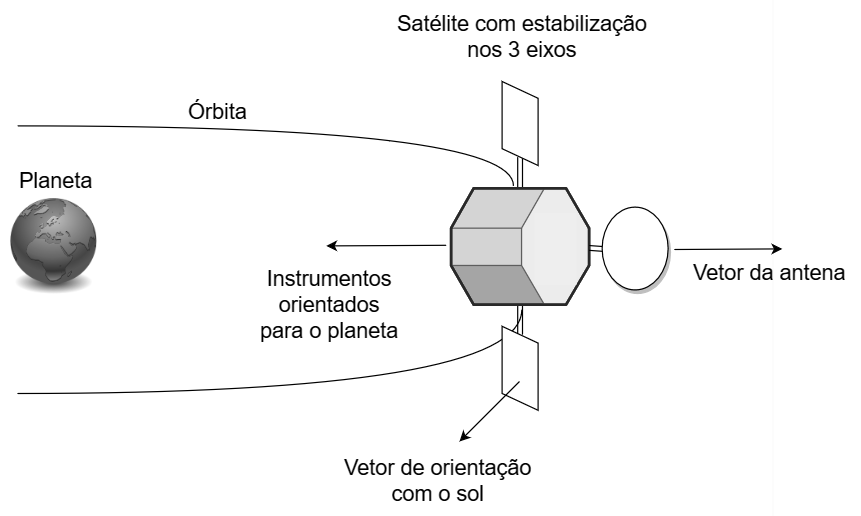
\includegraphics[scale=0.5]{referencial/img/rotational_brown_p256}
  \end{center}
  \fonte{Adaptado de \citeonline{Brown2002}.} 
  \label{fig:rotational_brown_p256}
\end{figure}

%%%%%%%%%%%%%%%%%%%%%%%%%%%%%%%%%%%

\subsection{Dinâmica de um Satélite}\label{cap:dinamica}

A dinâmica é dividida em duas partes, onde uma representa os movimentos de translação e a outra os de rotação.

A \textit{dinâmica de translação} de um copo em relação ao outro é um caso de \textit{Dinâmica de Corpo Rígido}. A fundação da Dinâmica de corpos rígidos foi feita pelo Físico Inglês Isaac Newton em forma de três leis, das quais, a 2º e a 3ª são primordiais para descrever a \textit{dinâmica de rotação} \cite{Snider}. A 2ª lei de Newton pode ser escrita das seguintes forma:

\begin{equation}\label{eq:fma}
  \vec{F}=\frac{d}{dt}\vec{p}\quad\quad\quad\quad\vec{p}=m\vec{v}
\end{equation}

\begin{equation}
  \vec{F}=m\vec{a}
\end{equation}

Onde $\vec{F}$ é a força, $\vec{p}$ é o momento linear, $\vec{v}$ é a velocidade e $\vec{a}$ é  aceleração. Ainda, podemos descrever a força total sobre uma partícula $\vec{F}_i$ da seguinte forma:

\begin{equation}\label{eq:Fi}
\vec{F}_i=\vec{f}_{ie}+\sum_{i\neq j}^{N}{\vec{f}_{ie}} = m_i\vec{a}_i
\end{equation}
 
 Onde, $\vec{f}_{ie}$ é a força externa e $\vec{f}_{ij}$ é a força interna de carda parte j que compõe o corpo i e $m_i\vec{a}_i$ é a massa e a força resultante no corpo rígido. Ao unirmos N partículas para formar um corpo rígido, estamos somando todas as forças externas e as forças internas de todos os corpos da seguinte forma:

\begin{equation}
  \sum_{i=1}^{N}{\vec{F}_i}=\sum_{i=1}^{N}{\vec{f}_i}+\sum_{i=1}^{N}{\sum_{i\neq j}^{N}{\vec{f}_ij=}}\sum_{i=1}^{N}{m_i\vec{a}_i} 
\end{equation}

Segundo a 3ª Lei de Newton, como o corpo j exerce uma força $\vec{f}_{ji}$ em módulo igual a força $\vec{f}_{ij}$ que o corpo i exerce sobre o corpo j, só que oposta. Logo, as forças internas se anulam. Quando temos um conjunto de partículas unidas, podemos descrever a força total sobre o corpo ($\vec{F}_e$) como o somatório de todas as forças sobre as partículas ($\vec{F}_{ie}$). Isso pode ser escrito da seguinte forma:

\begin{equation}\label{eq:fet}
  \vec{F}_{e}=\sum_{i=1}^{N}{\vec{f}_{ie}}=\sum_{i=1}^{N}{m_i\vec{a}_i} 
\end{equation}

A imagem \ref{fig:translacao_referencial_snider_p15}, representa o vetor posição $\vec{r_{com}}$ de um corpo rígido em relação a origem. A descrição matemática desse vetor pode ser visto na equação \ref{eq:rcom}.

\begin{figure}[H]
  \caption{Representação de $\vec{r}_{com}$}
  \begin{center}
      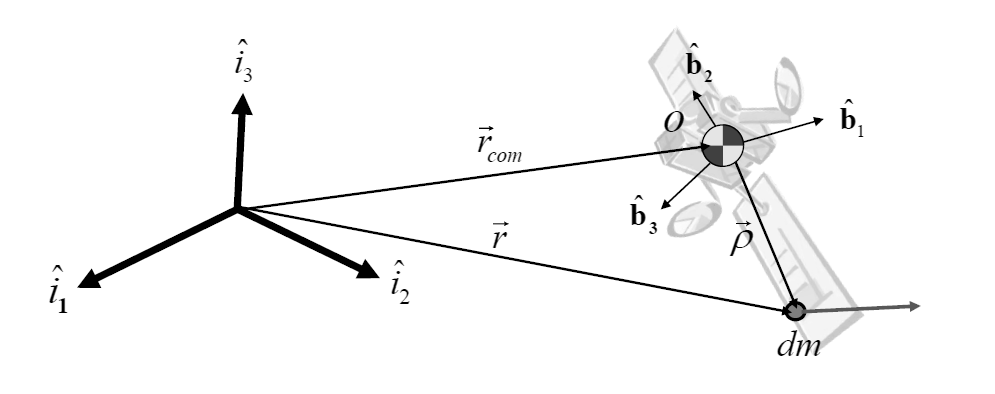
\includegraphics[scale=0.5]{referencial/img/translacao_referencial_snider_p15}
  \end{center}
  \fonte{Adaptado de \citeonline{Snider}.} 
  \label{fig:translacao_referencial_snider_p15}
\end{figure}

\begin{equation}\label{eq:rcom}
  \vec{r}_{com}=\frac{1}{M_T}\sum_{i=1}^{N}{m_i\vec{r}_i} 
\end{equation}

Onde, $M_T$ é a massa total do corpo rígido.

Como a aceleração é a derivada segunda da posição, derivamos duas vezes a posição $\vec{r}_{com}$ e multiplicamos pela massa total em ambos os lado da equação \ref{eq:rcom}. Assim temos:

\begin{equation}\label{eq:2deriv}
  M_T\frac{{d}^{2}}{{d}t^{2}}\vec{r}_{com}=\sum_{i=1}^{N}{m_i\vec{a_i}}
\end{equation}

Igualando as equações \ref{eq:fet} e \ref{eq:2deriv}, temos a força total sobre um corpo rígido que desempenha movimento de translação. Isso pode ser visto na sequência.

\begin{equation}
\vec{F_e}=M_{T}\frac{{d}^{2}}{{d}t^{2}}\vec{r}_{com}
\end{equation}

A \textit{dinâmica de rotação} descreve o movimento de um corpo rígido em relação a um ponto. Para descrevermos os movimentos de rotação, devemos conhecer a distribuição de massa do corpo rígido \cite{Snider}. A figura \ref{fig:mass_snider_p16} ilustra a distribuição de massa infinitesimal de um corpo tridimensional. Por definição, o momento de inércia infinitesimal disposto sobre um eixo ($I_{xx}$, $I_{yy}$ e $I_{zz}$) é o produto da massa pela distância do ponto de referência. Se fizermos isso para N partículas, temos:

\begin{figure}[H]
  \caption{Distribuição de massa.}
  \begin{center}
      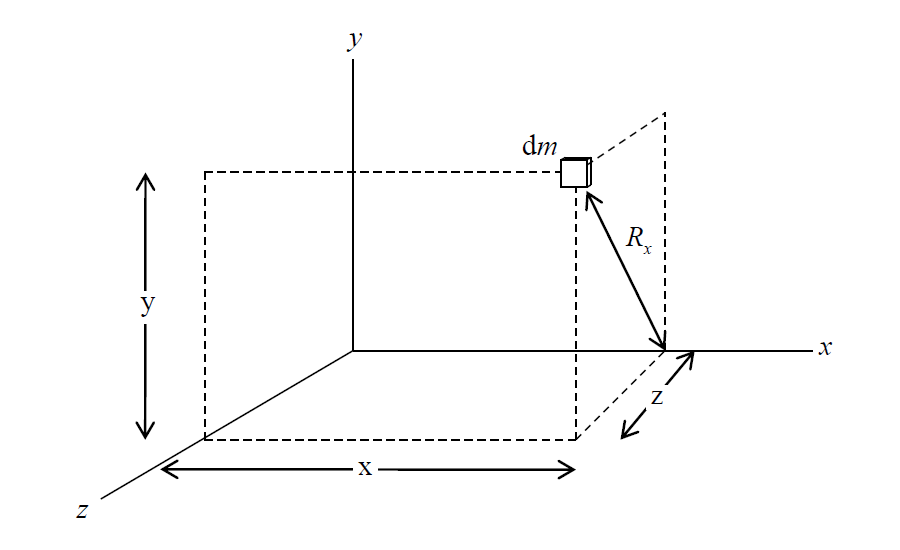
\includegraphics[scale=0.5]{referencial/img/mass_snider_p16}
  \end{center}
  \fonte{Adaptado de \citeonline{Snider}.} 
  \label{fig:mass_snider_p16}
\end{figure}

\begin{equation}
  I_{xx}=\sum_{i=1}^{N}{m_i({y_i}^{2}+{z_i}^{2})}
\end{equation}

\begin{equation}
  I_{yy}=\sum_{i=1}^{N}{m_i({x_i}^{2}+{z_i}^{2})}
\end{equation}

\begin{equation}
  I_{zz}=\sum_{i=1}^{N}{m_i({x_i}^{2}+{y_i}^{2})}
\end{equation}

Já quando as partículas estão dispostas sobre os planos xy, xz e yz, temos:

\begin{equation}
  I_{xy}=-\sum_{i=1}^{N}{m_ix_iy_i}=I_{xy}
\end{equation}

\begin{equation}
  I_{xz}=-\sum_{i=1}^{N}{m_ix_iz_i}=I_{zx}
\end{equation}

\begin{equation}
  I_{yz}=-\sum_{i=1}^{N}{m_iy_iz_i}=I_{zy}
\end{equation}

Com isso, podemos criar uma matriz que representa o momento de inércia total do corpo rígido:

\begin{equation}\label{eq:nsimetrico}
I=\begin{bmatrix}I_{xx}&I_{xy}&I_{xz}\\I_{yx}&I_{yy}&I_{yz}\\I_{zx}&I_{zy}&I_{zz}\end{bmatrix}
\end{equation}

Caso o satélite seja simétrico, os momentos de inércia nos planos xy, xz e yz são de mesmo módulo só que com sinal oposto aos momentos de inércia dos planos xy, zx e zy, anulando todos esses termos. Isso pode ser visto na seguinte matriz diagonal:

\begin{equation}
I=\begin{bmatrix} I_{ xx } & 0 & 0 \\ 0 & I_{ yy } & 0 \\ 0 & 0 & I_{ zz } \end{bmatrix}=\begin{bmatrix} A & 0 & 0 \\ 0 & B & 0 \\ 0 & 0 & C \end{bmatrix}
\end{equation}

Para facilitar a escrita das equações, os momentos de inércia $I_{xx}$, $I_{yy}$ e $I_{zz}$ serão descritos como A, B e C respectivamente. Após a descrição matemática do momento de inércia, podemos começar a analisar o movimento de rotação do corpo rígido. Vamos começar pela velocidade angular instantânea $\omega$, que pode ser descrita como a derivada primeira da posição $\beta$ angular, segundo o teorema fundamental do cálculo:

\begin{equation}
\omega\equiv\lim_{\Delta t\rightarrow 0}\frac{\Delta\beta}{\Delta t}=\frac{d\beta}{dt}
\end{equation}

A aceleração angular $\alpha$, nada mais é do que a primeira derivada da velocidade angular:

\begin{equation}
\alpha\equiv\lim_{\Delta t\rightarrow 0}\frac{\Delta\omega}{\Delta t}=\frac{d\omega}{dt}
\end{equation}

Outra equação importante para descrever a maioria dos tipos de movimento, é aquela que relaciona a posição $\beta$ com a posição inicial $\beta_0$, velocidade angular inicial $\omega_0$, o tempo inicial do movimento $t_0$, o tempo atual t e a aceleração angular $\alpha$. A expressão pode ser vista na sequência.

\begin{equation}
\beta=\beta_{0}+\omega_{0}(t-t_{0})+\frac{1}{2}\alpha{(t-t_{0})}^{2}
\end{equation}

Não menos importante, é a expressão que relaciona a velocidade angular $\omega$ com a velocidade angular inicial $\omega_0$, aceleração angular e o deslocamento ($\beta-\beta_0$). Isso é descrito na equação da sequência.

\begin{equation}
{\omega}^{2}={\omega_0}^{2}+2\alpha(\beta-\beta_0) 
\end{equation}

Como foi feito na dinâmica de translação, precisamos relacionar os momentos e a aceleração angular $\alpha$. Para isso vamos começar relacionando o torque $\vec{\tau}$ com a derivada do momento angular $\vec{L}$:

\begin{equation}
\vec{\tau}=\dot{\vec{L}}
\end{equation}

Mas como o momento angular é o produto do momento de inércia do corpo I pela velocidade angular, assim: 

\begin{equation}\label{eq:iomega}
\vec{L}=I\vec{\omega}
\end{equation}

Com isso, já conhecendo as relações entre velocidade e aceleração, temos:  

\begin{equation}\label{iomega}
\vec{\tau}=I\dot{\vec{\omega}}=I\vec{\alpha}
\end{equation}

Se usarmos o teorema do transporte cinemático, o momento de inércia pode ser escrito da seguinte forma:

\begin{equation}
\dot{\vec{L}}=I\dot{\vec{\omega}}+\vec{\omega}\times I \vec{\omega}
\end{equation}

Por consequência, descrevemos o torque da seguinte maneira:

\begin{equation}\label{eq:torque}
\vec{\tau}=I\dot{\vec{\omega}}+\vec{\omega}\times I \vec{\omega}
\end{equation}

Como temos o momento de inércia do corpo rígido representado em forma de matriz, precisamos mudar a representação a matricial. Começaremos pela velocidade angular $\vec{\omega}$, que em módulo, pode ser descrita da seguinte forma:

\begin{equation}
\left|\vec{\omega}\right|=\begin{bmatrix}\omega_1\\\omega_2\\\omega_2\end{bmatrix}
\end{equation}

Se fizermos o mesmo com a equação \ref{eq:torque}, temos:

\begin{equation}
\begin{bmatrix}\tau_{1}\\\tau_{2}\\\tau_{3}\end{bmatrix}=\begin{bmatrix}A\dot{\omega}_{1}\\B\dot{\omega}_{2}\\C\dot{\omega}_{3}\end{bmatrix}+\begin{bmatrix}\omega_{1}\\\omega_{2}\\\omega_{3}\end{bmatrix}\times\begin{bmatrix}A\omega_{1}\\B\omega_{2}\\C\omega_{3}\end{bmatrix}
\end{equation}

Como podemos ver, já conseguimos relacionar os momentos de inércia do corpo rígido simétrico com as demais variáveis de interesse. Além disso, podemos sair da forma matricial e apresentarmos os torques da forma algébrica, isso pode ser visto nas 3 equações a seguir.

\begin{equation}
  \tau_1=A\dot{\omega_1}-(B-C)\omega_2\omega_3 
\end{equation}

\begin{equation}
  \tau_2=B\dot{\omega_2}-(C-A)\omega_1\omega_3 
\end{equation}

\begin{equation}
  \tau_3=C\dot{\omega_3}-(A-B)\omega_1\omega_2
\end{equation}

Se utilizarmos um corpo não simétrico, podemos recorrer a matriz da equação \ref{eq:nsimetrico}, e obteremos as 3 seguintes equações para descrever o torque:

\begin{equation}\label{eq:torquexyz}
 \tau_{1}=I_{xx}\dot{\omega_{1}}-I_{xy}(\dot{\omega_{2}}-\omega_{1}\omega_{3})-I_{xz}(\dot{\omega_{3}}+\omega_{1}\omega_{2})\\-(I_{yy}-I_{zz})\omega_{2}\omega_{3}-I_{yz}({\omega_{2}}^{2}-{\omega_{3}}^{2})
\end{equation}

\begin{equation}\label{eq:torquexyz2}
  \tau_{2}=I_{zz}\dot{\omega_{3}}-I_{yz}(\dot{\omega_{3}}-\omega_{1}\omega_{2})-I_{xy}(\dot{\omega_{1}}+\omega_{2}\omega_{3})\\-(I_{zz}-I_{xx})\omega_{1}\omega_{3}-I_{xz}({\omega_{3}}^{2}-{\omega_{1}}^{2})
\end{equation}

\begin{equation}\label{eq:torquexyz3}
 \tau_{3}=I_{zz}\dot{\omega_{1}}-I_{xz}(\dot{\omega_{1}}-\omega_{2}\omega_{3})-I_{yz}(\dot{\omega_{2}}+\omega_{1}\omega_{3})\\-(I_{xx}-I_{yy})\omega_{1}\omega_{2}-I_{xy}({\omega_{1}}^{2}-{\omega_{2}}^{2})
\end{equation}

Se isolarmos a derivada da velocidade angular na nas equações \ref{eq:torquexyz}, \ref{eq:torquexyz2} e \ref{eq:torquexyz3}, temos:

\begin{equation}
  \dot{\omega_{1}}=\frac{\tau_{1}}{A}+\left(\frac{B-C}{A}\right)\omega_{2}\omega_{3}
\end{equation}

\begin{equation}
  \dot{\omega_{2}}=\frac{\tau_{2}}{B}+\left(\frac{C-A}{B}\right)\omega_{1}\omega_{3}
\end{equation},

\begin{equation}
  \dot{\omega_{3}}=\frac{\tau_{2}}{C}+\left(\frac{A-B}{C}\right)\omega_{1}\omega_{2}
\end{equation}

Assim conseguimos a relação da velocidade com o torque aplicado. Essa é uma expressão que representa a reação em forma de variação de velocidade que um torque provoca.


%%%%%%%%%%%%%%%%%%%%%%%%%%%%%

\subsubsection{Rodas de Reação}

Uma roda de reação consiste em um dispositivo que é fixado em um eixo de motor, com o objetivo de interferir na posição de um corpo através da variação de velocidade angular das rodas. Quando a roda sofre uma variação da sua velocidade angular, ela exerce um torque em uma determinada direção \cite{BongWie2001}. Esse efeito ocorre devido à conservação do momento angular do corpo, logo, se a roda está sendo desacelerada, o corpo tende se opor a esse movimento. Na figura \ref{fig:satellite_controlhand_p1306} podemos ver 3 rodas de reação dispostas nos 3 eixos de um corpo rígido.

\begin{figure}[H]
  \caption{Representação simplificada de um corpo rígido com rodas de reação.}
  \begin{center}
      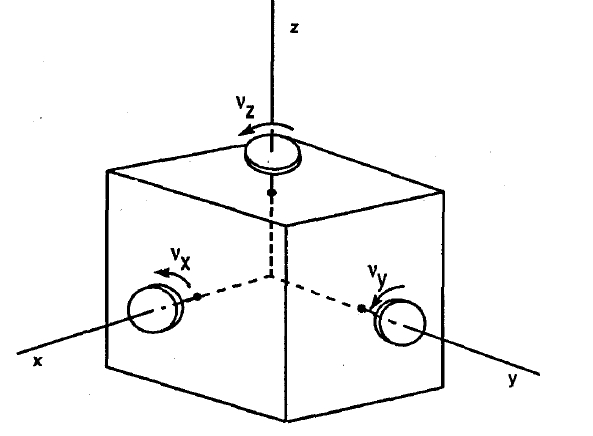
\includegraphics[scale=0.65]{referencial/img/satellite_controlhand_p1306}
  \end{center}
  \fonte{Adaptado de \citeonline{Levine1996}.} 
  \label{fig:satellite_controlhand_p1306}
\end{figure}

Como já foram descritos nas outras seções, precisamos encontrar uma relação que expresse o torque criado pelas rodas de reação, para que consigamos unir ao modelo do satélite. Para isso, começamos pelo momento angular total $\vec{L}_{total}$, que pode ser visto na sequência:

\begin{equation}\label{eq:ltot}
\vec{L}_{total}=\vec{L}_s+\vec{L}_{\omega}=constante 
\end{equation}

Onde $L_s$ representa o momento angular do satélite e $\vec{L}_{\omega}$ o momento angular da roda de reação. Como já vimos na equação \ref{eq:iomega}, o momento angular pode ser descrito da seguinte forma:

\begin{equation}
\vec{L}_s=I\vec{\omega}
\end{equation}

E o momento angular nas rodas de ração pode ser escritos da seguinte forma:

\begin{equation}
\vec {L}_{\omega} =J_{\omega}\vec{\psi}_{\omega}
\end{equation}

Onde $J_{\omega}$ é o momento de inércia da roda de reação e $\vec{\psi}_{\omega}$ é variação instantânea da posição angular da roda. Com isso, conseguimos encontrar o torque provido pela roda de reação $\tau_{\omega}$:

\begin{equation}\label{eq:torqueedo}
\vec{\tau}_{\omega}=\dot{\vec{L}}_{\omega}=J_{\omega}\dot{\vec{\psi}}_{\omega}
\end{equation}

E por fim, podemos relacionar as velocidades angulares do satélite com o as inércia e as velocidades das rodas da seguinte forma:

\begin{equation}\label{eq:modeloA}
  \dot{\omega_{1}}=\frac{J_{\omega 1}\dot{\vec{\psi}}_{\omega 1}}{A}+\left(\frac{B-C}{A}\right)\omega_{2}\omega_{3}
\end{equation}

\begin{equation}\label{eq:modeloB}
  \dot{\omega_{2}}=\frac{J_{\omega 2}\dot{\vec{\psi}}_{\omega 2}}{B}+\left(\frac{C-A}{B}\right)\omega_{1}\omega_{3}
\end{equation},

\begin{equation}\label{eq:modeloC}
  \dot{\omega_{3}}=\frac{J_{\omega 3}\dot{\vec{\psi}}_{\omega 3}}{C}+\left(\frac{A-B}{C}\right)\omega_{1}\omega_{2}
\end{equation}

Para isso é usada a equação \ref{eq:ltot} e a relação entre torque e momento angular da equação \ref{eq:torqueedo}. Assim, temos a última equação que faltava para descrever toda a dinâmica de um satélite artificial simétrico. 


%%%%%%%%%%%%%%%%%%%%%%%%%%%%%%%%%%%%%%%%%%%%%%%%%%%%%%%%%%%%%%%%%%%%%%

\section{Controladores PID}

Como já temos as equações diferenciais que descrevem o modelo satélite, precisamos desenvolver os conceitos básicos de controle para controlarmos as variáveis de interesse. Esses conceitos estão descritos nas próximas seções


%%%%%%%%%%%%%%%%%%%%%%%%%%%%%%%%%%%

\subsection{Resposta ao Degrau do um Sistema}

Um problema fundamental em engenharia, é prever e modelar sistemas naturais ou artificias para tirarmos o melhor proveito de suas características. Para isso, muitas técnicas foram desenvolvidas para se conseguir controlar essas variáveis de interesse \cite{Levine1996}.

Uma forma clássica de representar uma resposta de uma variável de interesse, é através da resposta ao degrau. Essa pode ser vista na figura \ref{fig:transient_ogata_p170}, onde temos as principais características da resposta ao degrau de um sistema de segunda ordem ou superior. Onde \textit{$M_p$} (maximum overshoot) é o sobressinal da variável de interesse em percentual, \textit{$t_d$} (Delay Time) é o tempo atraso de transporte, \textit{$t_r$} (rise time) é o tempo necessário para atingir o valor do sinal de referência, \textit{$t_p$} é o tempo de pico (peak time) e \textit{$t_s$} (settling time) é o tempo para o sistema entrar em regime, observando um critério de erro em regime \cite{Ogata}.

\begin{figure}[H]
  \caption{Parâmetros de uma resposta ao degrau de um sistema de segunda ordem ou superior.}
  \begin{center}
      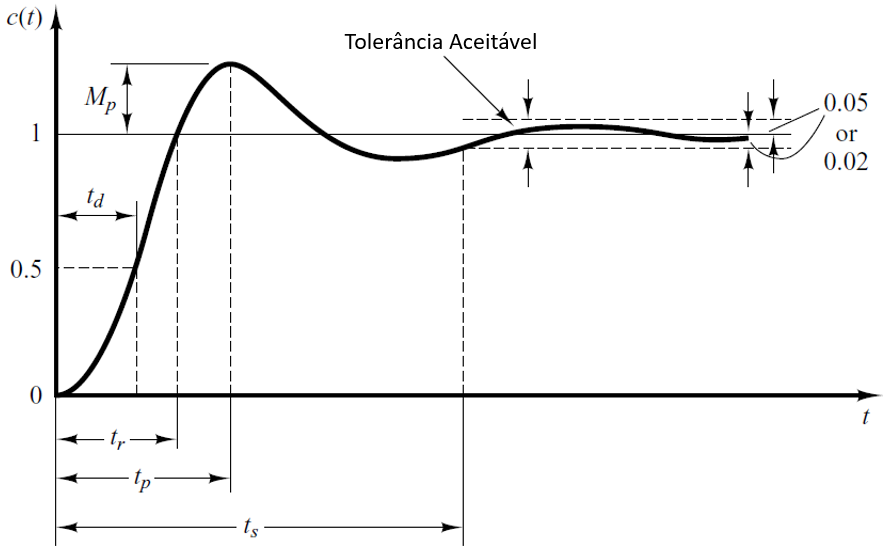
\includegraphics[scale=0.5]{referencial/img/transient_ogata_p170}
  \end{center}
  \fonte{Adaptado de \citeonline{Ogata}.} 
  \label{fig:transient_ogata_p170}
\end{figure}

A resposta ao degrau nos diz muito sobre os sistemas de interesse, pois nela podemos ver claramente a atuação dos \textit{polos} e \textit{zeros} dominantes e o ganho de baixa frequência da função de transferência do sistema. Os métodos clássicos para se calcular os parâmetros de controladores são baseados na resposta ao degrau \cite{Ogata}. 


%%%%%%%%%%%%%%%%%%%%%%%%%%%%%%%%%%%

\subsection{Controlador PID}

O controlador proporcional-integral-derivativo é um dos controladores mais utilizados nas aplicações industriais. Essa topologia de controlador consegue, em diferentes configurações atender entre 90 e 95\% de todos os sistemas que necessitam de controladores \cite{Levine1996}. A forma descritiva matemática mais comum de se encontrar um controlador PID no domínio do tempo é a seguinte:

\begin{equation}\label{eq:PID}
  u(t) = K\left((e(t)+\frac{1}{T_i}\int_{0}^{t}{e(\tau)}d\tau+T_d\frac{de(t)}{dt}\right) 
\end{equation}

Onde \textit{e(t)} é o erro, \textit{$T_i$} é o tempo integral, \textit{$T_d$} é o tempo derivativo e \textit{K} o ganho proporcional. Uma outra forma de se representar os tempos integral e derivativo, é através dos ganhos \textit{$K_i$} que é o ganho integral e o \textit{$K_d$}, que é o ganho derivativo \cite{Astrom1995}.s

Na figura \ref{fig:pid_controller_Snider_p35}, podemos ver a configuração mais utilizada do controlador PID, onde $\beta_{com}(S)$ é o valor do sinal de referência no domínio da frequência, \textit{err(S)} o erro, \textit{$K_p$} é o ganho proporcional, \textit{$K_i$} é o ganho integral, \textit{$K_d$} é o ganho derivativo, \textit{D(S)} é um distúrbio, \textit{$G_p(S)$} é a função de transferência da planta e por fim, \textit{$\beta(S)$} que é a variável de interesse \cite{Snider}.

\begin{figure}[H]
  \caption{Representação do modelo de controlador PID com distúrbios.}
  \begin{center}
      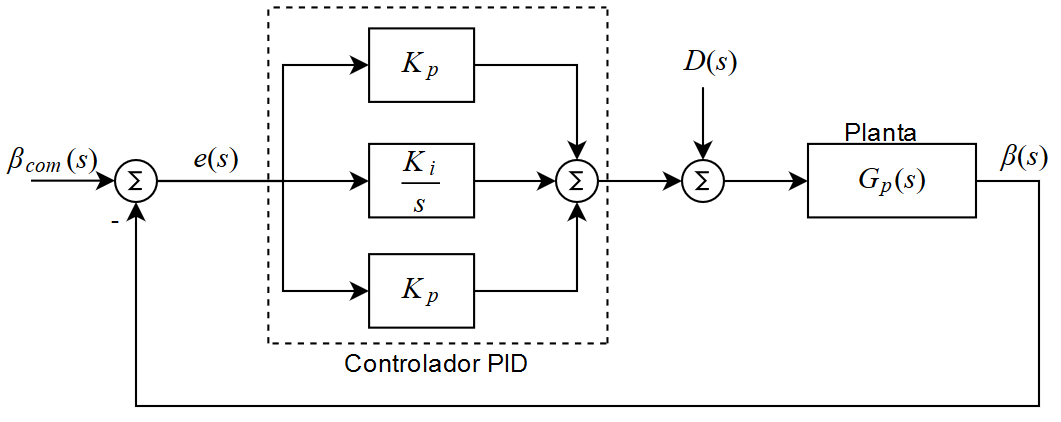
\includegraphics[scale=0.55]{referencial/img/pid_controller_Snider_p35}
  \end{center}
  \fonte{Adaptado de \citeonline{Snider}.} 
  \label{fig:pid_controller_Snider_p35}
\end{figure}

Como alguns sistemas podem admitir grandes e rápidas variações de sinais de referência, exigindo uma grande força de controle e energia no atuador, algumas topologias foram desenvolvidas para limitar a atuação de alguns fatores dos controladores. Um bom exemplo é o \textit{anti-windup}, onde essa topologia limita a saturação do atuador quando o sistema atinge o regime, causado pela ação integral. Essa topologia pode ser vista no modelo da figura \ref{fig:pid_antiwindup_astrom_p83} \cite{Astrom1995}.

\begin{figure}[H]
  \caption{Modelo de um controlador PID com histerese.}
  \begin{center}
      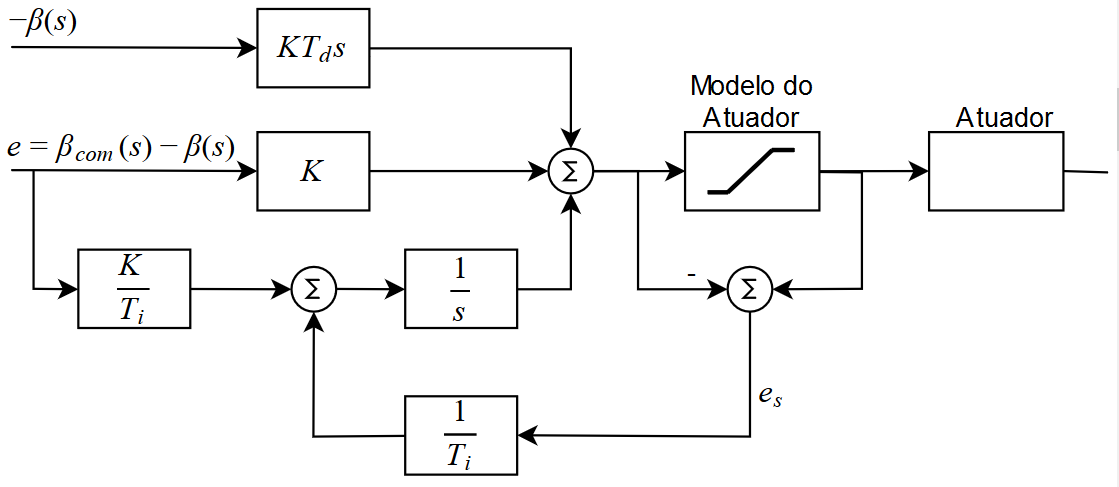
\includegraphics[scale=0.55]{referencial/img/pid_antiwindup_astrom_p83}
  \end{center}
  \fonte{Adaptado de \citeonline{Astrom1995}.} 
  \label{fig:pid_antiwindup_astrom_p83}
\end{figure}

Existem muitas combinações de controladores PID, cada uma com suas peculiaridades e vantagens de uso. Uma combinação muito usada é a PI, onde a acão integral de zerar o erro em regime e uma boa resposta transitória já satisfazem as especificações. 


%%%%%%%%%%%%%%%%%%%%%%%%%%%%%%%%%%%

\subsection{Controle Digital}

Quando utilizamos um dispositivo digital como controlador, temos que representar os sinais de forma discretizada, ou seja, em níveis que possam ser transformados em um conjunto de bits. Só assim o microcontrolador ou microprocessador poderá realizar as operações matemáticas desejadas. Para essa transformação, usamos coversores AD (analógico-digital) que convertem um sinal analógico (contínuo) em um sinal binário \cite{BongWie2001}. Um sinal analógico é representado digitalmente com um período T, da seguinte forma:

\begin{equation}
  y(0), y(T), y(2T), ...
\end{equation}

Se expressarmos usando notação ${y[kT]}$, podemos representar uma equação diferencial da seguinte forma:

\begin{equation}
  u(k) = a_{0}y[k]+a_{1}y[k-1]+...+a_{n}y[k-n] - b_{1}y[k-1] - b_{2}y[k-2] - ... -b_{n}y[k-n]
\end{equation}

Onde u(k) denota o sinal computado e y(k) os valores o sinal analógico nos instante k-ésimos.


%%%%%%%%%%%%%%%%%%%%%%%%%%%%%%%%%%%

\subsubsection{Transformada Z}

A transformada z é usada para aquisição e processamento de dados em sistemas discretos. Ela possui relação matemática com o domínio s da seguinte forma:

\begin{equation}
Z = e^{-Ts}
\end{equation}

Por definição, a transformada z é um somatório do produto de $z^{-k}$ com o valor do sinal analógico amostrado no momento k, y(k). Isso pode ser conferido na equação as seguir.

\begin{equation}
  y(z) \sum_{k=0}^{\infty}{y[k]z^{-k}} = y[0] + y[1]z^{-1}+y[2]z^{-2}...
 \end{equation} 

 Se usarmos os Teoremas da Tradução, Valor Inicial e Valor Final, conseguimos expressar uma função da seguinte forma \cite{BongWie2001}:

\begin{equation}
  \frac{u(z)}{y(z)} = \frac{a_0 + a_1z^{-1}+...+a_nz^{-n}}{1+b_1z^{-1}+b_2z^{-2}+...++b_nz^{-n}}
\end{equation}


%%%%%%%%%%%%%%%%%%%%%%%%%%%%%%%%%%%

\subsubsection{Amostragem}

Em um sistema discreto, uma forma de amostrar um sinal analógico é usar um trem de impulsos com amplitude do sinal y(t) nos tempos T e reter esses dados com um ZOH (Zero-Order-Hold - Amostrador de Ordem Zero). A figura \ref{fig:zoh_wie_p155} representa muito bem esse processo.

\begin{figure}[H]
  \caption{Conversão de um sinal contínuo em discreto.}
  \begin{center}
      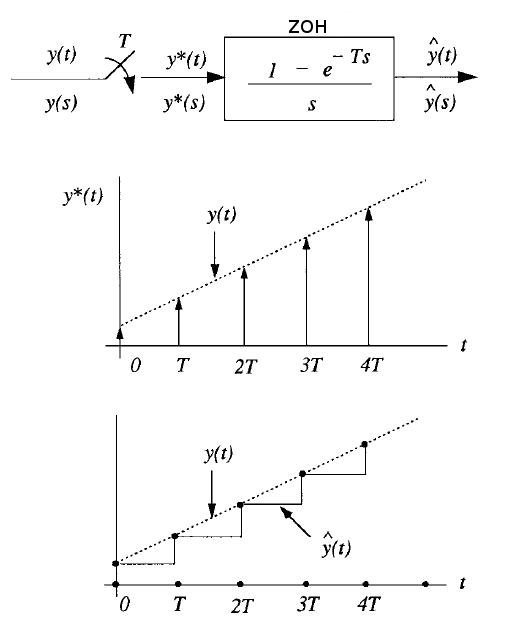
\includegraphics[scale=0.65]{referencial/img/zoh_wie_p155}
  \end{center}
  \fonte{Adaptado de \citeonline{BongWie2001}.} 
  \label{fig:zoh_wie_p155}
\end{figure}

Onde y(t) é o sinal que está sendo amostrado, y*(t) é o trem de pulsos amostrados e $\hat{y}(t)$ é o sinal resultante. Um ZOH ideal pode ser representando da seguinte forma:

\begin{equation}
  \hat{y}(s) \approx \frac{1-e^{-Ts}}{Ts}y(s)
\end{equation}

Essa expressão é de suma importância para a aquisição das variáveis que queremos controlar usando técnicas digitais.


%%%%%%%%%%%%%%%%%%%%%%%%%%%%%%%%%%%

\subsubsection{Controlador PID Digital}

Agora, desejamos descrever a representação do controlador PID da equação \ref{eq:PID} de forma discreta, para isso devemos usar a aproximação de Euler:

\begin{equation}
  s = \frac{1-z^{-1}}{T}
\end{equation}

Conseguimos expressar o controlador PID no domínio z da seguinte forma:

\begin{equation}
  u(t) = -K\left[1 + \frac{1}{T_i}\frac{T}{1-z^{-1}} + T_d\frac{1-z^{-1}}{T} \right]e(t)
\end{equation}

Com isso, podemos representar de forma discreta o controlador PID, isso pode ser visto na equação da sequência:

\begin{equation}\label{eq:pid_equation}
  u(t) = -K_p\left[y[k]-\frac{1}{T_i}{\hat{u}[k]}-T_d\frac{y[k]-y[k-1]}{T}\right]
\end{equation}

Onde

\begin{equation}
  \hat{u}[k] = \hat{u}[k-1] +Ty[k]
\end{equation}

Desse modo, concluímos a modelagem de um controlador PID, com um conjunto de equações que podem ser, de forma simples, implementadas em um sistema digital.


%%%%%%%%%%%%%%%%%%%%%%%%%%%%%%%%%%%

\subsubsection{Filtro de Kalman}

Quando se trabalha na aquisição de grandezas físicas, encontramos ruídos nos sinais amostrados. Esses ruídos podem inviabilizar o controle de uma planta, pois não informam o verdadeiro estado do sinal amostrado, fazendo com que o atuador atue de forma equivocada, levando a instabilidade o sistema. Uma forma de minimizar esse efeito, é utilizando o filtro de Kalman.

Filtro de Kalman é um algoritmo usado para estimar estados de variáveis de um sistema, sujeito a ruídos estocásticos. Esse algoritmo relaciona as informações sobre a dinâmica da planta e informações sobre o comportamento estocástico do dos sinais para estimar variáveis de estados da planta \cite{Levine1996}. Na figura \ref{fig:kalman_levine_p591}, temos a representação em diagrama de blocos do filtro de Kalman.

\begin{figure}[H]
  \caption{Diagrama de blocos do filtro de Kalman.}
  \begin{center}
      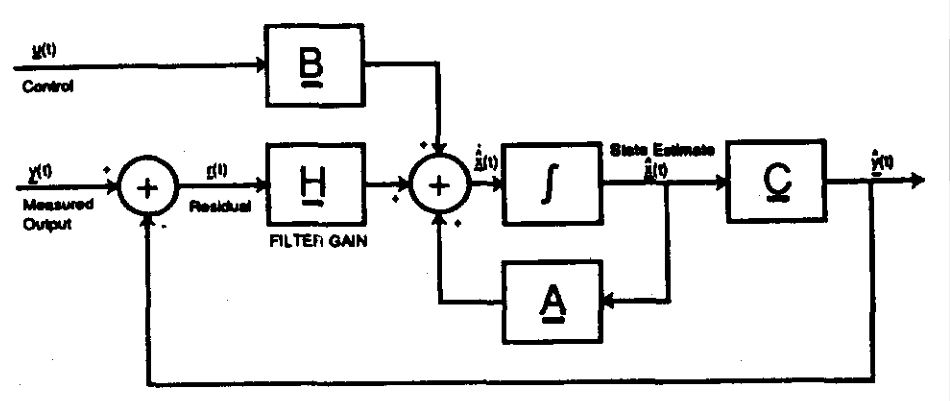
\includegraphics[scale=0.5]{referencial/img/kalman_levine_p591}
  \end{center}
  \fonte{Adaptado de \citeonline{Levine1996}.} 
  \label{fig:kalman_levine_p591}
\end{figure}

Onde $u(t)$ é o sinal do controlador, $y(t)$ é o sinal amostrado da saída da planta, $\hat {y}(t) $ é a saída estimada, H é o ganho do filtro e A, B e C são as matrizes em espaço de estados da dinâmica da planta.


%%%%%%%%%%%%%%%%%%%%%%%%%%%%%%%%%%%%%%%%%%%%%%%%%%%%%%%%%%%%%%%%%%%%%%

\section{Sintonia de Controladores}

Como podemos ver no modelo matemático e gráfico dos controladores PID, os valores de ajuste $K_p$, $T_i$ e $T_d$  podem assumir infinitos valores, sendo necessário a escolha do melhor conjunto desses valores para que a planta desempenhe o comportamento esperado \cite{Ogata}.


%%%%%%%%%%%%%%%%%%%%%%%%%%%%%%%%%%%

\subsection{Método de sintonia de Ziegler-Nichols}

Dois métodos clássicos de sintonia foram desenvolvidos em 1942 por Ziegler e Nichols. Esses dois métodos são baseados em características da resposta ao degrau e com a resposta em frequência. Na figura \ref{fig:ziegler-nichols_astrom_p135} podemos ver a resposta ao degrau e os parâmetros de atraso (L) e velocidade da resposta (a), que são usados para o cálculos dos parâmetros do controlador  \cite{Astrom1995}. 

\begin{figure}[H]
  \caption{Resposta ao degrau e seus parâmetros.}
  \begin{center}
      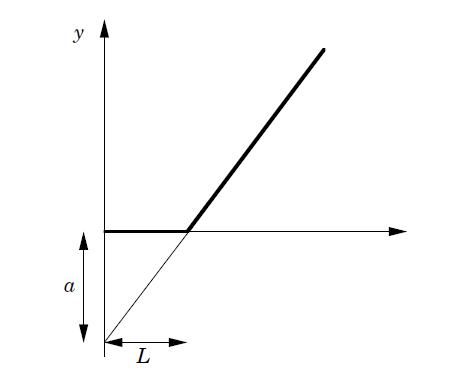
\includegraphics[scale=0.75]{referencial/img/ziegler-nichols_astrom_p135}
  \end{center}
  \fonte{\citeonline{Astrom1995}.} 
  \label{fig:ziegler-nichols_astrom_p135}
\end{figure}

Na tabela \ref{tab:Ziegler-Nichols} podemos ver as relações dos parâmetros $K_p$, $T_i$, $T_d$ e $T_p$ com os vistos na figura \ref{fig:ziegler-nichols_astrom_p135}. O outro método de se estimar os valores do controlador, é através de duas características da resposta em frequência: uma delas que é o ganho que deixa o sistema marginalmente estável ($K_u$), e a outra, é o período do sinal de referência que deixa o sistema marginalmente estável ($T_u$). Podemos ver na tabela \ref{tab:Ziegler-Nichols-freq} as relações entre $K_p$, $T_i$, $T_d$, $T_p$ e ($K_u$) e ($T_u$).

\begin{table}
  \caption{Parâmetros PID pelo método de Ziegler-Nichols - resposta ao degrau}
  \label{tab:Ziegler-Nichols}
  \centering%
  \begin{minipage}{.42\textwidth}
    \begin{tabular*}{\textwidth}{lllll}
      \hline
      {Controlador} & {K} & {$T_i$} & {$T_d$}& {$T_p$}\\ \hline
      \hline
      P    &  1/a   &     &      & 4L  \\ 
      PI   &  0.9/a & 3L  &      & 5.7L  \\
      PID  &  1.2/a & 2L  & L/2  & 3.4L  \\ \hline
    \end{tabular*}
    \fonte{Adaptado de \citeonline{Astrom1995}}
  \end{minipage}
\end{table}


\begin{table}
  \caption{Parâmetros PID pelo método de Ziegler-Nichols - resposta em frequência}
  \label{tab:Ziegler-Nichols-freq}
  \centering%
  \begin{minipage}{.52\textwidth}
    \begin{tabular*}{\textwidth}{lllll}
      \hline
      {Controlador} & {K} & {$T_i$} & {$T_d$}& {$T_p$}\\ \hline
      \hline
      P    &  0.5$K_u$   &           &             & $T_u$  \\ 
      PI   &  0.4$K_u$   & 0.8$T_u$  &             & 1.4$T_u$ \\
      PID  &  0.6$K_u$   & 0.5$T_u$  & 0.125$T_u$  & 0.85$T_u$  \\ \hline
    \end{tabular*}
    \fonte{Adaptado de \citeonline{Astrom1995}}
  \end{minipage}
\end{table}


%%%%%%%%%%%%%%%%%%%%%%%%%%%%%%%%%%%%%%%%%%%%%%%%%%%%%%%%%%%%%%%%%%%%%%

\subsection{Sintonia Automática de Controladores}

Como muitos sistemas sofrem variações temporais, distúrbios e o interesse do usuário em modificar constantemente a resposta da planta, cria-se a necessidade de automatizar o processo de sintonia, ao um simples comando do usuário. Além da simplicidade do conceito de implementação, os controladores PID são muito utilizados pela possibilidade de auto sintonia e adaptatividade dos controladores, pois a partir do comportamento da resposta ao degrau, podemos calcular os parâmetros do controlador e aplicarmos sem a intervenção humana\cite{Astrom1995}. Na figura \ref{fig:escolha_controle_astrom_p236}, podemos a partir do comportamento da planta, escolher a ou as técnicas mais adequadas que devemos implementar para controlar de forma satisfatória a planta.

\begin{figure}[H]
  \caption{Fluxograma para a escolha do método de sintonia.}
  \begin{center}
      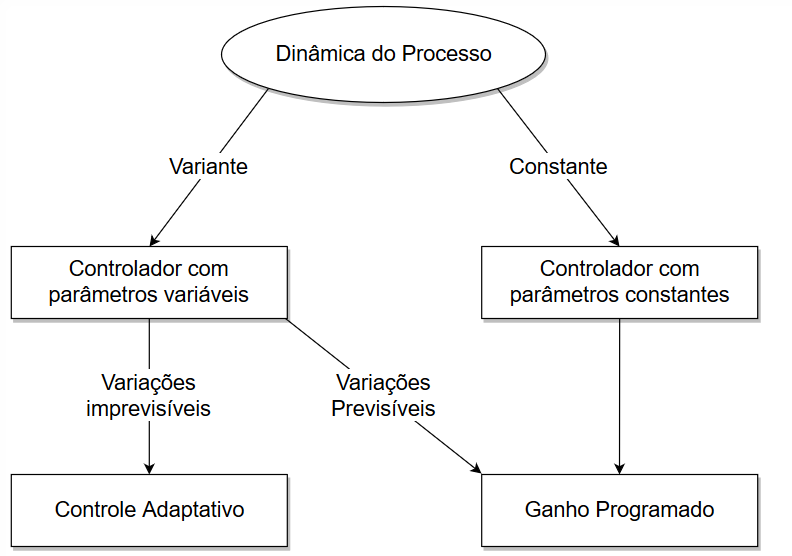
\includegraphics[scale=0.55]{referencial/img/escolha_controle_astrom_p236}
  \end{center}
  \fonte{Adaptado de \citeonline{Astrom1995}.} 
  \label{fig:escolha_controle_astrom_p236}
\end{figure}

Uma alternativa possível para sintonia de controladores, é o método do relé, ele, no modo clássico, se encontra entre os controladores com parâmetros constantes.


%%%%%%%%%%%%%%%%%%%%%%%%%%%%%%%%%%%

\subsubsection{Método do Relé}

Características da resposta em frequência podem ser descobertas se somarmos ao sinal de referência, uma onda retangular ao mesmo tempo em que o controlador PID está desconectado. Esse é o princípio do método de sintonia usando relé, onde o relé desempenha o papel do chaveamento e cria um sinal retangular sobreposto ao sinal de referência \cite{Levine1996}. Na imagem \ref{fig:pid_autotuning_relay_astrom_p239} podemos ver o conceito básico do método do relé. O modelo matemático usado para descrever o comportamento de um relé, pode ser visto na equação \ref{eq:n(a)} que está na sequência.
 
\begin{figure}[H]
  \caption{Modelo do método de auto sintonia via relé.}
  \begin{center}
      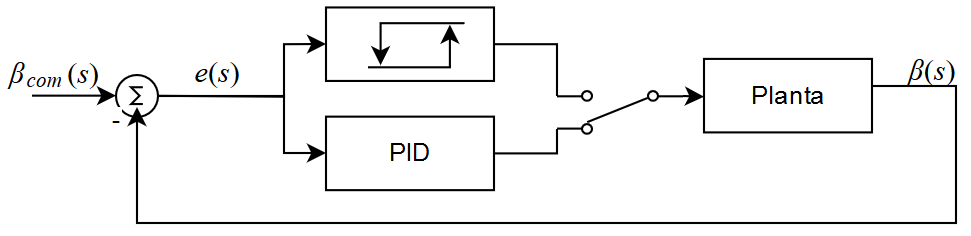
\includegraphics[scale=0.55]{referencial/img/pid_autotuning_relay_astrom_p239}
  \end{center}
  \fonte{Adaptado de \citeonline{Astrom1995}.} 
  \label{fig:pid_autotuning_relay_astrom_p239}
\end{figure}

\begin{equation}\label{eq:n(a)}
  N(a)=\frac{4d}{\pi a}\left(\sqrt{1-\left(\frac{\varepsilon}{a}\right)^{2}}-i\frac{\varepsilon}{a}\right) 
\end{equation}

Onde \textit{d} é a amplitude de oscilação do relé (normalmente até 10\% do sinal de referência), \textit{$\varepsilon$} é a histerese do relé e \textit{$a_r$} é a amplitude do sinal de referencia \cite{Levine1996}. Com isso, podemos calcular os parâmetros intermediários para a sintonia do controlador da seguinte forma:

\begin{equation}
  K_u \approx \frac{4d}{\pi a_r}
\end{equation}

Onde $T_u$ é o período de oscilação do sinal de interesse. Munido desses valores, podemos recorrer a tabela do método Ziegler-Nichols em resposta em frequência (Tabela \ref{tab:Ziegler-Nichols-freq}).


%%%%%%%%%%%%%%%%%%%%%%%%%%%%%%%%%%%%%%%%%%%%%%%%%%%%%%%%%%%%%%%%%%%%%%

\section{Estado da Arte - Controladores Inteligentes}

O estado da arte dentro de controle, está na criação de controladores inteligentes. Controle inteligente implementa conceitos de inteligência de organismos biológicos em forma de algoritmos. Esses algoritmos são usados para automatizar os processos de sintonia, promover a adaptação do controle perante as mudanças que a planta possa apresentar ou otimizar os parâmetros atuais. As duas principais formas de controle inteligente utilizadas na atualidade, são a por \textit{algoritmos genéticos} e \textit{por redes neurais}, onde a por redes neurais será explicada na sequência.


%%%%%%%%%%%%%%%%%%%%%%%%%%%%%%%%%%%

\subsection{Controle com Redes Neurais Artificiais}  %control hand p1017

Uma \textit{Rede Neural} (RNA) é um modelo matemático generalizado da cognição humana ou de um organismo biológico. O elemento básico de uma RNA é o neurônio, que associado em camada, forma uma rede de neurônios. Um neurônio pode ter n entradas e p saídas, e dentro de uma mesma camada, todos os neurônios devem ser idênticos. O processo de cognição é caracterizado como um comportamento não-linear, a função ($f_{rn}$) que descreve a excitação um neurônio binário unipolar,  pode ser vista na sequência \cite{Unal2013}. 

\begin{equation} \label{eq:neuron}
f(rn) \equiv \frac{1}{1+e^{-\lambda_n}}
\end{equation}

também

\begin{equation}
f(rn) \equiv sgn(rn) = \begin{Bmatrix}  1, \quad rn>0 \\ 1, \quad rn<0  \end{Bmatrix}
\end{equation}

Onde $\lambda_n$ é o ganho do neurônio. Uma representação gráfica de um neurônio natural comparado com um artificial pode ser visto na figura \ref{fig:neuronio_unal_p6}, onde os dendritos são representados pelas entradas $p_1, p_2, ..., p_R$, uma soma dessas entradas que posteriormente é aplicada a função da equação \ref{eq:neuron}, onde obtemos a saída $a$.

\begin{figure}[H]
  \caption{Célula de um neurônio natural e modelo matemático respectivo.}
    \begin{center}
        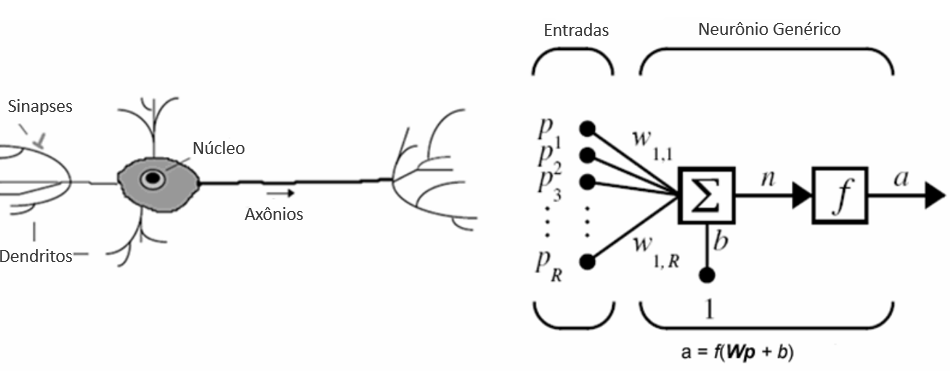
\includegraphics[scale=0.45]{referencial/img/neuronio_unal_p6}
  \end{center}
  \fonte{Adaptado de  \citeonline{Unal2013}.} 
  \label{fig:neuronio_unal_p6}
\end{figure}

Ao paralelizarmos um grupo de neurônios, criamos uma camada de neurônios, cada elemento dessa camada é conectado em todas as entradas, ou em todos os neurônios da camada anterior, ou posterior, ou ainda, nas saídas. Uma representação de uma rede neural pode ser vista na figura \ref{fig:feedforward_neural_astrom_p297}, onde temos 5 entradas ($u_1,...,u_5$) e duas saídas ($y_1 y_2$).

\begin{figure}[H]
  \caption{Representação de uma rede neural.}
  \begin{center}
      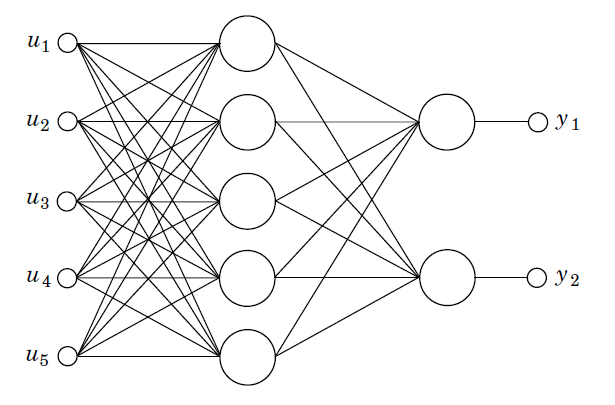
\includegraphics[scale=0.5]{referencial/img/feedforward_neural_astrom_p297}
  \end{center}
  \fonte{Adaptado de \citeonline{Astrom1995}.} 
  \label{fig:feedforward_neural_astrom_p297}
\end{figure}

Em controle, as RNAs são usadas principalmente em sistemas não lineares, onde existem regiões que a planta não é controlável pelas técnicas de controle clássicas \citeonline{Chen2004}. Nesse caso, a RNA recebe os sinais de controle do controlador e da saídas da planta, realiza as operações e encontra os novos parâmetros para o controlador PID. Um bom exemplo dessa topologia pode ser visto na figura \ref{fig:pid_neural_chen_p212}, onde os parâmetros obtidos pela rede neural ainda são linearizados para que sejam utilizados pelo controlador.

\begin{figure}[H]
  \caption{Controlador PID com rede neural.}
  \begin{center}
      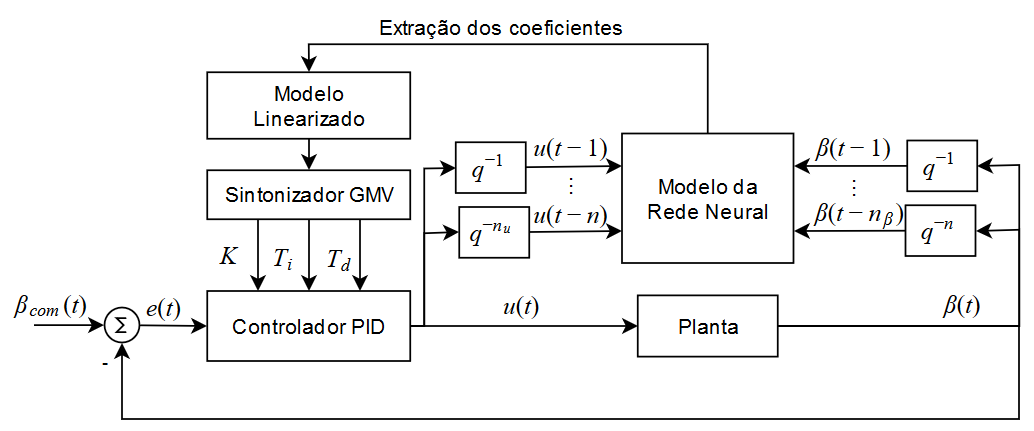
\includegraphics[scale=0.55]{referencial/img/pid_neural_chen_p212}
  \end{center}
  \fonte{Adaptado de \citeonline{Chen2004}.} 
  \label{fig:pid_neural_chen_p212}
\end{figure}

Na imagem anterior, existe o GMV (General Minimum Variance - Variância Mínima Geral) que é usado para extrair os parâmetros $K$ $T_i$ $T_d$ do modelo da rede neural linearizada \citeonline{Chen2004}.


%#########################

\subsubsection{Regressão Não-Linear Robusta}

Regressão é um método matemático para o ajuste de curva através da otimização de parâmetros que compõem a equação característica do sinal. O caso de interesse, é a regressão para sinais não-lineares, os quais são provenientes da RNA, que precisarão ser otimizados sobre a equação característica do controlador PID (equação \ref{eq:pid_equation}). De forma genérica, a equação que descreve um modelo não-linear pode ser descrita da seguinte forma \cite{robust2019}:

\begin{equation}
 y_i = f(x_i; \theta_e) + \epsilon_i, \quad\quad i = 1,...,n
\end{equation}

Onde $y_i$ é a resposta observável, $x_i$ é o vetor k-dimensional com os valores conhecidos e $\theta_e$ é p-dimensional com valores desconhecidos que influenciam a reposta observável e $\epsilon_i$ é o erro que satisfaz alguma regularidade estocástica. 

Um dos métodos mais usados para regressão, independente da linearidade do sistema, é o \textit{Método dos mínimos quadrados} (MMQ), que pode ser representado da seguinte forma:

\begin{equation}
 S(\theta_e) = \sum_{i=1}^{n}[y_i-f(x_i;\theta_e)]^2 
\end{equation}

Esse método por definição, é usado onde as amostras obedecem uma distribuição normal. Quando isso não é verdadeiro, usa-se o método MMQ robusto, onde o erro pode assumir outras distribuições mantando a boa resposta da regressão. Na figura \ref{fig:robust_regression}, podemos ver a comparação entre os métodos MMQ e MMQ Robusto, ficando clara a melhor resposta do MMQ Robusto.

\begin{figure}[H]
  \caption{Comparação entre os métodos de regressão não-lineares.}
  \begin{center}
      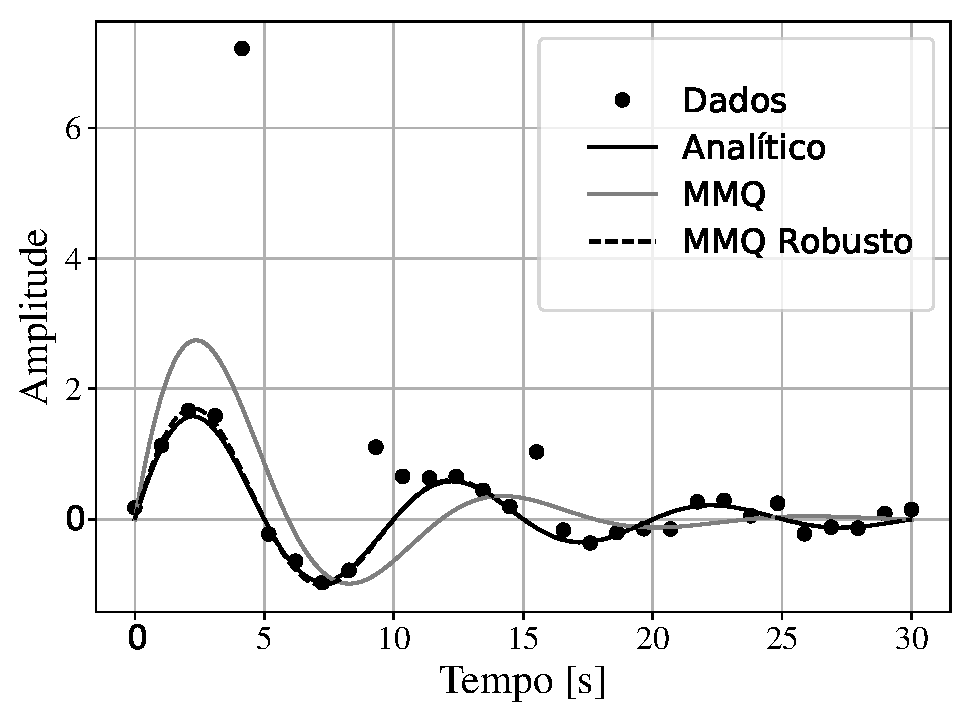
\includegraphics[scale=0.7]{referencial/img/robust_regression}
  \end{center}
  \fonte{Adaptado de \citeonline{RegressionPython}.} 
  \label{fig:robust_regression}
\end{figure}

Os últimos itens abordados, apontam algumas das modernas técnicas aplicadas em controle, as quais aplicarei no presente trabalho de forma conjunta, propondo uma técnica afim para a sintonia de controladores. Após elucidados os conceitos básicos para a realização do trabalho, todos os passos para a implementação da mecânica, do software e o sistema de controle serão descritos no próximo capítulo. 
\chapter{Metodologia}

A metodologia do presente trabalho é dividida em três principais partes. A primeira é a etapa de projeto dos componentes mecânicos que fazem parte do satélite, entre eles: as rodas de reação, motor DC (\textit{Direct Current} - corrente contínua), mancal a ar e hastes. Também contempla as especificação dos componentes eletrônicos que constituem o satélite. É na segunda etapa que ocorre a modelagem completa do sistema e especificações das limitações de movimentação do satélite, juntamente com a elaboração dos diagramas de blocos do controle. Nessa etapa também é feita a modelagem do motor DC, para que possa fornecer torque para tirar da inércia a planta. Já na terceira etapa, são abordados os elementos de \textit{software}, de rede e supervisão do satélite. Nessa etapa também se encontram as especificações e o desenvolvimento do \textit{software} de controle e supervisão.


%%%%%%%%%%%%%%%%%%%%%%%%%%%%%%%%%%%%%%%%%%%%%%%%%%%%%%%%%%%%%%%%%%%%%%

\section{Hardware}

Após a modelagem apresentada no referencial teórico, é possível modelar um simulador de satélite de fabricação factível.  O mancal a ar, a base de suporte do simulador do satélite, rodas de reação, motores \textit{Brushless} (motor de corrente contínua sem escovas) e os outros elementos, podem ser vistos na figura \ref{fig:satelite_completo}.

\begin{figure}[H]
  \caption{Desenho mecânico completo do simulador de satélite.}
  \begin{center}
      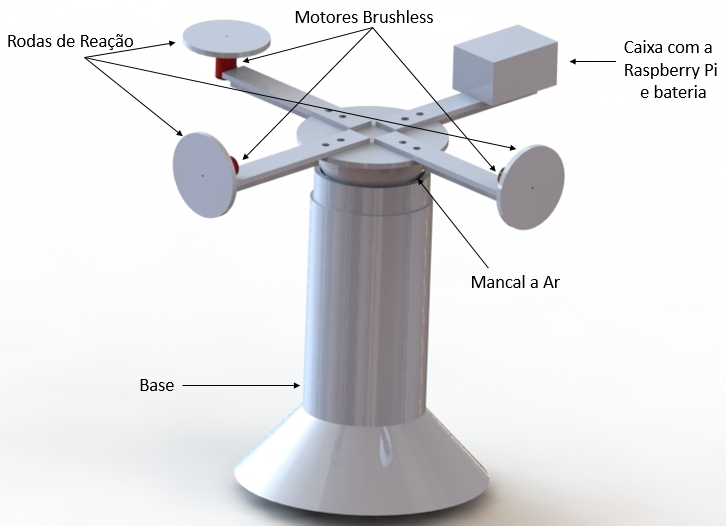
\includegraphics[scale=.5]{metodologia/img/satelite_completo}
  \end{center}
  \fonte{Elaborado pelo Autor.} 
  \label{fig:satelite_completo}
\end{figure}

 Como podemos ver na imagem anterior, o modelo sofre várias simplificações em relação a um satélite real, onde o modelo passa a ser de fácil implementação, possibilitando a validação dos conceitos propostos nesse trabalho. Dentre várias simplificações, a mais óbvia, o simulador não apresentará de forma direta os movimentos de translação descritos no seção \ref{cap:dinamica}. Ainda, existe uma limitação para os ângulos $\phi$, $\theta$ e $\psi$ que é um intervalo de $0<\phi, \theta, \psi<240º$ devido a existência do mancal a ar e a simetria do corpo do satélite, como princípio para simplificar a modelagem matemática do mesmo. Os principais elementos do simulador de satélites, serão descritos de forma detalhada na sequência, dentre eles, o corpo do satélite.


%%%%%%%%%%%%%%%%%%%%%%%%%%%%%%%%%%%

\subsection{Corpo do Simulador de Satélite}

O elemento de dinâmica mais importante que deve ser dimensionado, é o corpo do satélite. É nele que são fixados todos os outros elementos que compõem o simulador de satélites. Para isso, optamos como material, o alumínio, pois possui menor densidade e resistência mecânica adequada para o projeto. Na figura abaixo podemos ver o corpo do simulador.

\begin{figure}[H]
  \caption{Corpo do simulador de satélites.}
  \begin{center}
      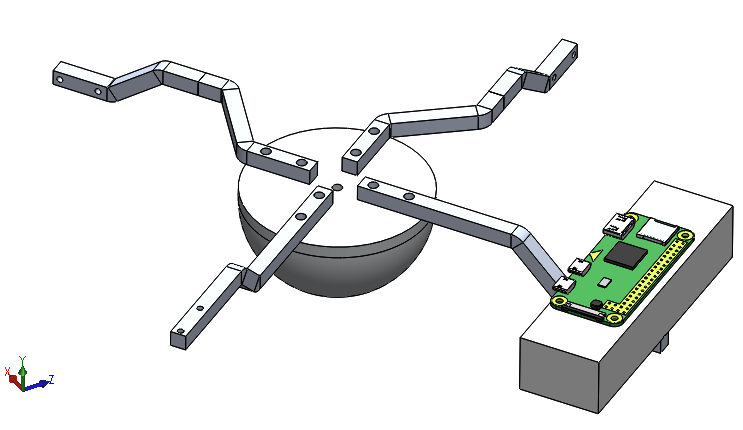
\includegraphics[scale=.4]{metodologia/img/corpo_satelite}
  \end{center}
  \fonte{Elaborado pelo Autor.} 
  \label{fig:corpo_satelite}
\end{figure}


Onde \textit{hx} é a haste do motor que atua no eixo x, \textit{hy} é a haste do motor que atua no eixo y, \textit{hz} é a haste do motor que atua no eixo z, \textit{hb} é a haste da bateria e \textit{se} é a semiesfera que é a interface entre o corpo e o mancal a ar. Esse último, apresenta explicação na sequência. O projeto leva em consideração a distribuição de massa e os centros de massa, pois o simulador de satélite deve ficar o mais simétrico e em equilíbrio possível, facilitando a atuação do controle que prevê sua simetria.

Através do \textit{software} de desenho mecânico SolidWorks\copyright, onde o projeto foi desenvolvido, conseguimos calcular o peso do satélite, que é de aproximadamente $\SI{1,25}{\kg}$, contado com a bateria de polímero de Lítio e outro periféricos. Esse valor é necessário para o dimensionamento das rodas de reação, que também será descrito na sequência. Ainda, com o mesmo \textit{software}, conseguimos os valores de momento de inércia máximo entre os eixos, que é de aproximadamente $\SI{0,5}{\kg\meter\squared}$, o qual é usado para dimensionamento das rodas de reação.


%%%%%%%%%%%%%%%%%%%%%%%%%%%%%%%%%%%

\subsection{Mancal a Ar}

Um dos elementos mais importantes do simulador, é o mancal a ar. Ele possibilita a criação mínima de atrito entre a esfera e a região côncava, pois existe um fluxo de ar promovido por um sistema pneumático que cria uma camada de ar entre as duas partes. Com isso, a esfera fica com movimento praticamente livre de atritos dentro de uma região limitada pela geometria da esfera, o corpo do satélite, a massa do satélite e a pressão do sistema pneumático. O modelo mecânico do mancal com seus elementos podem ser vistos na figura \ref{fig:base_desenho}.

\begin{figure}[H]
  \caption{Desenho mecânico do mancal a ar.}
  \begin{center}
      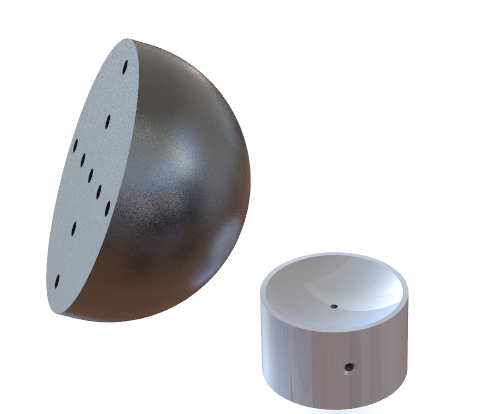
\includegraphics[scale=.4]{metodologia/img/base_desenho}
  \end{center}
  \fonte{Elaborado pelo Autor.} 
  \label{fig:base_desenho}
\end{figure}

O mancal precisou ser usinado, devido à precisão do encaixe entre a esfera e a região concava, para que a camada de ar seja o mais homogênea possível, evitando turbulências e regiões com atrito maiores que em outras. 


%%%%%%%%%%%%%%%%%%%%%%%%%%%%%%%%%%%

\subsection{Motor DC e Rodas de Reação}

Como foi descrito no referencial, os atuadores do satélite serão rodas de reação acopladas em motores de corrente contínua (DC). Na sequência, são descritos os cálculos das rodas de reação e a escolha dos motores DC. 


\subsubsection{Projeto das Rodas de Reação}

Partindo do princípio da conservação do momento angular do corpo do satélite, precisamos dimensionar o momento angular da roda e, por consequência, os momentos de inércia delas. Para isso, precisamos calcular o momento angular do satélite, que pode ser descrito como:

\begin{equation}
\vec{L_s} = 2\left(I_{sat} + m\left(\frac{r_{sat}}{2}\right)^2\right)  
\end{equation}

Cada roda é responsável por um terço do momento angular total do satélite, como pode ser visto na sequência:

\begin{equation}
\vec{L}_{roda} = \frac{\vec{L}_s}{3}   
\end{equation}

Onde $I_{sat}$ é o momento de inércia do satélite, $m$ é a massa, $r_{sat}$ é a distância dos motores em relação ao centro de massa. Podemos relacionar o momento angular com o momento de inércia das rodas e a velocidade angular, como podemos ver abaixo.

\begin{equation}
\vec{L}_{roda} = I_{roda}\vec{\omega}_{roda}
\end{equation}

Conseguimos dimensionar o momento angular das rodas através da variação do momento de inércia ou rotação das rodas. Com o objetivo de controlar o satélite, varia-se a velocidade angular das rodas com momento de inércia fixo. Na figura \ref{fig:motor_roda_desenho2}, temos o desenho escolhido para o projeto das rodas, pois, concentramos mais massa na extremidade, contribuindo assim, para um maior momento de inércia.

\begin{figure}[H]
  \caption{Geometria básica para o projeto de rodas de reação.}
  \begin{center}
      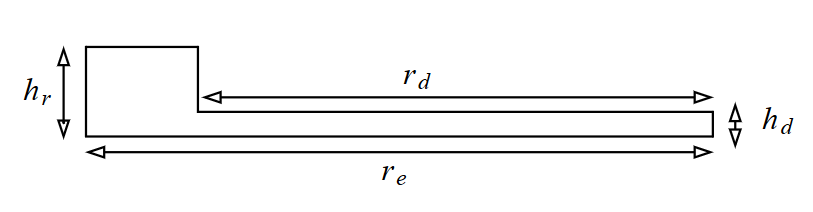
\includegraphics[scale=.45]{metodologia/img/roda_reacao_modelo}
  \end{center}
  \fonte{Elaborado pelo Autor.} 
  \label{fig:motor_roda_desenho2}
\end{figure}

Essa geometria escolhida, possui momento de inércia que pode ser descrito pela seguinte equação:

\begin{equation}
\vec{I}_{roda} = \rho \frac{\pi}{2}(h_r(r_{e}^4-r_d^4)+h_dr_d^4) 
\end{equation}

Onde $\vec{I}_{roda}$ é o momento de inércia da roda, $\rho$ é a densidade do material que compõe a roda, $h_r$ é a espessura da borda, $h_d$ é a espessura do disco, $r_e$ é o raio total da roda e $r_d$ é o raio do disco. Um conjunto de parâmetros que satisfazem as equações acima descritas à uma velocidade angular de $\SI{230.38}{\radian\per\second}$(2200 RPM) pode ser visto na tabela \ref{tab:react}. 

\begin{table}[H]
  \caption{Dimensões das rodas de reação.}
  \label{tab:react}
  \centering%
  \begin{minipage}{.42\textwidth}
    \begin{tabular*}{\textwidth}{cc}
      \hline
      {Dimensão} & Unidade \\ \hline
      \hline
      $\rho$  &  $\SI{7860}{\kilogram\per\cubic\metre}$ (Aço SAE 1045)\\ 
      $h_r$   &  $\SI{10.5}{\milli\metre}$ \\
      $h_d$   &  $\SI{2}{\milli\metre}$  \\
      $r_e$   &  $\SI{37}{\milli\metre}$  \\
      $r_d$   &  $\SI{30}{\milli\metre}$  \\ \hline
    \end{tabular*}
    \fonte{Elaborado pelo Autor.} 
  \end{minipage}
\end{table}

Com isso, concluímos o projeto da roda de reação, agora, passamos para a etapa do projeto do motor, que está na sequência.


%%%%%%%%%%%%%%%%%%%%%%%%%%%%%%%%%%%

\subsubsection{Escolha dos Motores DC}

O atuador do simulador de satélite é constituído de um conjunto de três motores \textit{Brushless} dispostos um em cada eixo cartesiano. Juntamente com esses motores, são acopladas rodas de reação, que farão os movimentos de rotação do satélite. Como exibido na imagem \ref{fig:satelite_completo}, os motores e as hastes estão distribuídos de forma simétrica e afastados do centro de massa do satélite, para facilitar a movimentação promovida pelo torque dos motores. O modelo de motor escolhido foi o \textit{Turnigy D2826-6 2200kV}, que é um motor usado em aeromodelos que possui relação de velocidade de 2200 RPM por Volt. Na imagem \ref{fig:motor_roda_desenho} podemos ver parte da haste, o motor e a roda de reação, todos acoplados. 

\begin{figure}[H]
  \caption{Desenho mecânico do conjunto motor-roda.}
  \begin{center}
      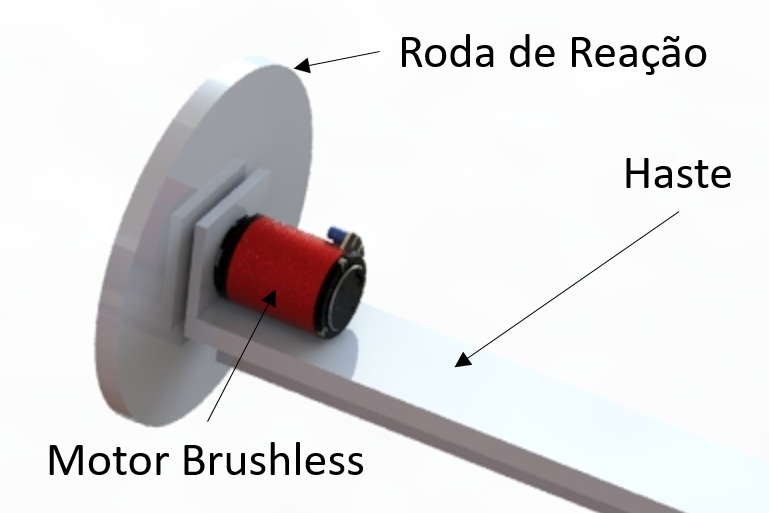
\includegraphics[scale=.45]{metodologia/img/motor_roda_desenho}
  \end{center}
  \fonte{Elaborado pelo Autor.} 
  \label{fig:motor_roda_desenho}
\end{figure}

A roda de reação também foi usinada, pois é necessário uma roda com uma massa e formato específico, para que possa ser acoplar ao motor e o conjunto consiga realizar os movimentos desejados. 


%%%%%%%%%%%%%%%%%%%%%%%%%%%%%%%%%%%

\subsection{Elementos Eletrônicos}

A placa de desenvolvimento e prototipação de sistemas embarcados Raspberry Pi Zero W (RPi) foi a escolhida, pois ela conta com os elementos mínimos de interfaceamento com os atuadores e outros periféricos. Além disso, ela possui conectividade \textit{wireless} (sem fio), possibilitando a supervisão e controle do satélite sem fio. Como o trabalho terá o seu desenvolvimento baseado em desenvolvimento de \textit{software} e adaptações do sistema operacional, uma placa com suporte, boa documentação e comunidade ativa, facilita o desenvolvimento. 

% Uma representação dessa placa pode ser vista na figura \ref{fig:rasp_zero}.

% \begin{figure}[H]
%   \caption{Raspberry Pi Zero W.}
%   \begin{center}
%       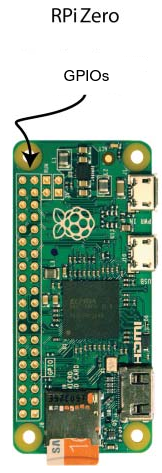
\includegraphics[scale=.55]{metodologia/img/rasp_zero}
%   \end{center}
%   \fonte{Adaptado de \citeonline{Molloy2016}} 
%   \label{fig:rasp_zero}
% \end{figure}

Um outro elemento que é indispensável, é o acelerômetro, o qual desempenha o papel de sensor de realimentação da posições angulares do satélite. Sua comunicação com a RPi é dada através da interface I2C, que está descrita na seção de \textit{software}. O giroscópio informará ao modelo a velocidade angular em graus por segundo, e o algoritmo calcula a posição através da integral da velocidade instantânea em cada eixo. Para isso, escolhemos o giroscópio MPU6050.

% \begin{figure}[H]
%   \caption{Placa de Circuito impresso com o acelerômetro e Giroscópio MPU6050.}
%   \begin{center}
%       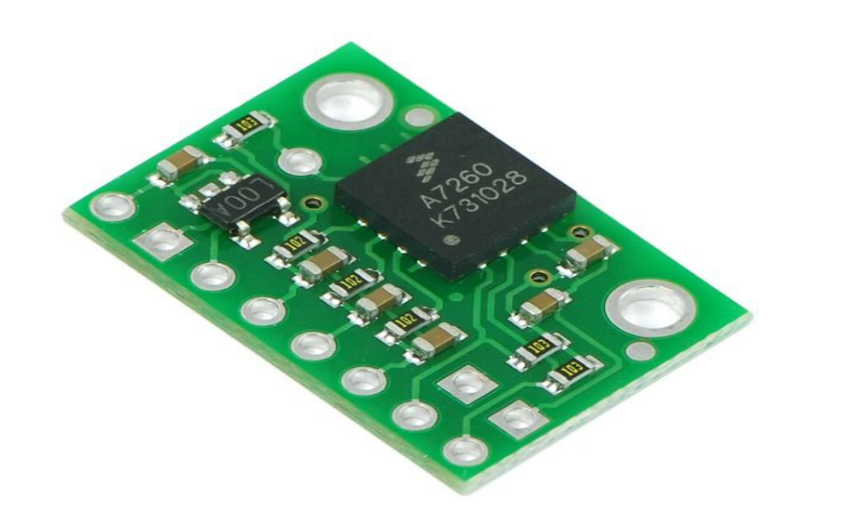
\includegraphics[scale=.35]{metodologia/img/pci_acelerometro_calache_p22}
%   \end{center}
%   \fonte{Adaptado de \citeonline{mpu}} 
%   \label{fig:pci_acelerometro_calache_p22}
% \end{figure}

Ainda, para o acionamento dos motores \textit{Brushless} serão utilizados ESC (\textit{Electronic-Speed-Control} - Controlador eletrônico de velocidade) que serão conectados com a bateria, os motores e a RPi. Após a conclusão do dimensionamento e escolha dos materiais, foi possível fazer a fabricação mecânica e montagem do simulador satélite, o qual pode ser visto nas figuras \ref{fig:base_real}, \ref{fig:corpo_real} e \ref{fig:simulador_real}.

\begin{figure}[H]
  \caption{Base do simulador de satélites prototipado.}
  \begin{center}
      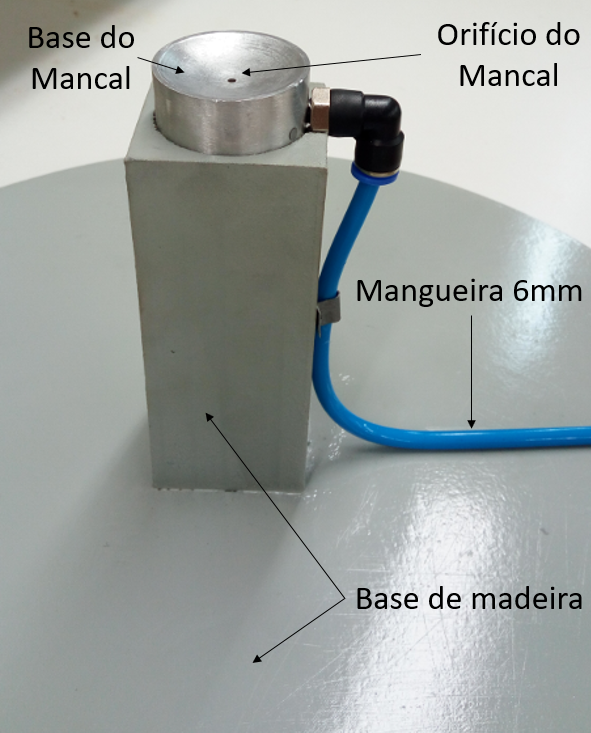
\includegraphics[scale=.5]{metodologia/img/base_real}
  \end{center}
  \fonte{Elaborado pelo Autor.} 
  \label{fig:base_real}
\end{figure}

Na imagem anterior, pode-se ver a base do simulador, feita em madeira, onde se encontram a região concava do mancal e as conexão 
pneumáticas. Já na figura \ref{fig:corpo_real}, podemos ver as partes que compõem o corpo do simulador.

\begin{figure}[H]
  \caption{Corpo do simulador de satélites prototipado.}
  \begin{center}
      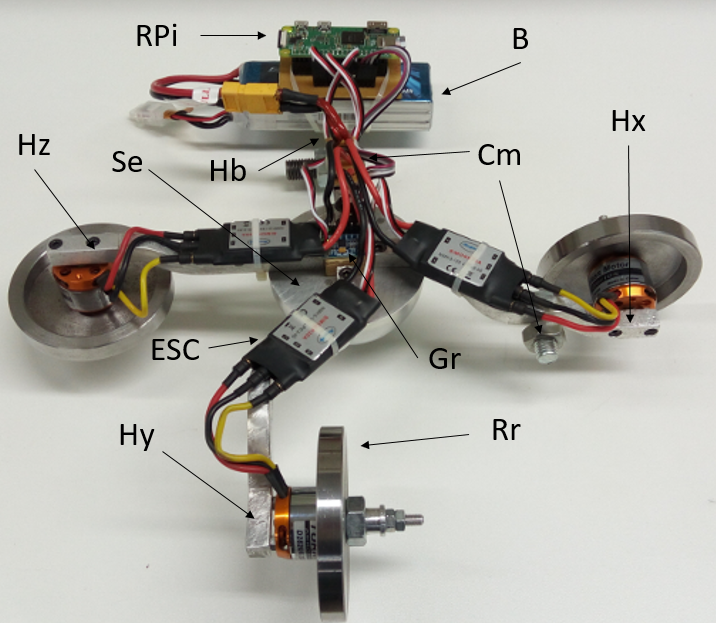
\includegraphics[scale=.7]{metodologia/img/corpo_real}
  \end{center}
  \fonte{Elaborado pelo Autor.} 
  \label{fig:corpo_real}
\end{figure}

Onde \textit{Rpi} é a Rapberri Pi Zero W, \textit{B} é bateria, \textit{ESC} são os dispositivos de acionamento dos motores brushles, \textit{Rr} são as rodas de reação, \textit{Cm} são massas para compensação de massa do simulador, \textit{Gr} é o acelerômetro/giroscópio, \textit{Se} é a semiesfera de alumínio que compõe o mancal, \textit{Hb} é a haste de alumínio da bateria, \textit{Hx} é a haste do motor do eixo x, , \textit{Hy} é a haste do motor do eixo y e \textit{Hz} é a haste do motor do eixo z. E por fim, a imagem completa do simulador de satélites, que pode ser vista na figura \ref{fig:simulador_real}.

\begin{figure}[H]
  \caption{Simulador de satélites prototipado.}
  \begin{center}
      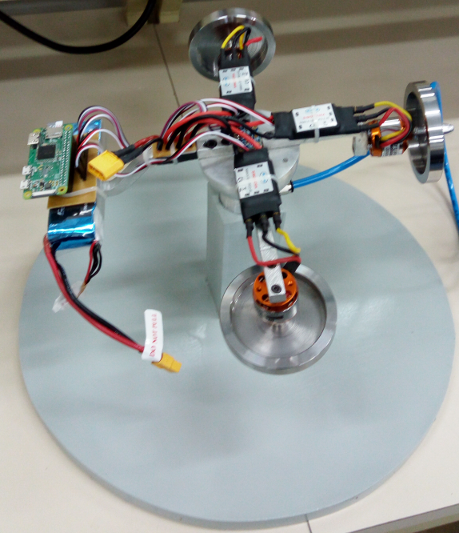
\includegraphics[scale=.65]{metodologia/img/simulador_real}
  \end{center}
  \fonte{Elaborado pelo Autor.} 
  \label{fig:simulador_real}
\end{figure}

Com isso, todos os principais elementos de hardware foram descritos, sendo a modelagem dos mesmos o próximo passo do desenvolvimento.


%%%%%%%%%%%%%%%%%%%%%%%%%%%%%%%%%%%%%%%%%%%%%%%%%%%%%%%%%%%%%%%%%%%%%%

\section{Sistemas de Controle}

Após a descrição dos conceitos básicos de controle e do modelo mecânico do satélite, é possível desenvolver os modelos da planta e do sistema de controle. Ainda nessa seção, é descrita a modelagem do motor de corrente contínua sugerido na seção anterior e posteriormente a modelagem completa do simulador de satélites.


%%%%%%%%%%%%%%%%%%%%%%%%%%%%%%%%%%%
\subsection{Modelo Motor DC}

Após a escolha do tipo de motor que será utilizado como atuador no controle da atitude do satélite, se faz necessário a modelagem do mesmo, para que consigamos acoplar ao modelo do satélite, o torque que promoverá a variação no momento angular do satélite, e por consequência, a posição angular. A figura \ref{fig:modelo_motor_dc} representa o modelo elétrico associado ao momento de inércia do rotor $J_{\omega 1}$ ao rotor e a da roda de reação $J_{\omega 2}$

\begin{figure}[H]
  \caption{Modelo do motor DC.}
  \begin{center}
      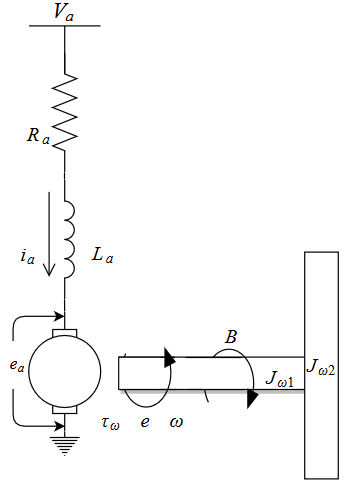
\includegraphics[scale=.7]{metodologia/img/modelo_motor_dc}
  \end{center}
  \fonte{Elaborado pelo Autor.} 
  \label{fig:modelo_motor_dc}
\end{figure}

Onde $R_a$, $L_a$, $i_a$ e $e_a$ são a resistência, a indutância, a corrente e a tensão de armadura, respectivamente, $e_b$ é a tensão induzida e $\tau_{\omega}$ é o torque do motor. A relação entre a corrente com a tensão de armadura pode ser vista na sequência \cite{Ogata}.

\begin{equation}
L_a \frac{di_a}{dt}+R_a i_a + e_b = e_a
\end{equation}

Como existe a relação entre a constante de torque $K_t$ e a tensão induzida, juntamente com a relação entre a constante de velocidade contra-eletromotriz $K_w$ e a tensão da fonte $V_a$. Isso pode ser visto na sequência.

\begin{equation}
  e_a = K_t\frac{d\theta}{dt}
\end{equation}

e

\begin{equation}
  e_b = K_wV_a
\end{equation}

Temos que:

\begin{equation}\label{eq:la}
L_a \frac{di_a}{dt}+R_a i_a + K_t\frac{d\theta}{dt} = K_wV_a
\end{equation}

Ainda, a relação que através do conceito de equilíbrio de torque, conseguimos relacionar o torque do motor $\tau_{\omega}$ com os momentos de inércia do rotor e da roda de reação com a corrente da armadura da seguinte forma:

\begin{equation}\label{eq:tauj}
\tau_{\omega} = (J_{\omega 1} + J_{\omega 2})\frac{d^{2}\theta}{dt^{2}}+B\frac{d\theta}{dt} = K_t i_a
\end{equation}

Onde B é o atrito viscoso. Como queremos relacionar a tensão da fonte com a velocidade angular, devemos manipular as equações \ref{eq:la} e \ref{eq:tauj} e aplicarmos a transformada de Laplace. O resultado dessas operações pode ser visto na sequência: 

\begin{equation}
  \frac{\omega(s)}{V_a(s)} = \frac{K_wK_t}{(R_a+ sLa)(s(J_{\omega 1} + J_{\omega 2})+B)+K_wK_t}  
\end{equation}

Mas como nas equações \ref{eq:modeloA}, \ref{eq:modeloB} e \ref{eq:modeloC} é necessário a a derivada instantânea da velocidade, ou seja, a aceleração do motor, precisamos derivar a equação anterior, e ainda, podemos dizer que a soma dos momentos de inércia é representado somente por $J$, obtendo assim:

\begin{equation}\label{eq:motor_accel}
  \frac{\dot{\omega}(s)}{V_a(s)} = \frac{K_wK_t s}{(R_a+ Las)(Js+B)+K_wK_t}  
\end{equation}

Com isso, modelamos o atuador do satélite, o próximo passo para a completa modelagem, é acoplar esse modelo com o do satélite descrito na seção \ref{cap:dinamica}. Esses passos serão descritos na próxima subseção.


%%%%%%%%%%%%%%%%%%%%%%%%%%%%%%%%%%%

\subsection{Modelo Completo do Satélite}

Como em partes, todo o satélite já foi modelado até agora, nessa subseção acoplaremos todos os modelos em um único, que terá como variável de interesse a posição angular tridimensional definida pelos ângulos $\psi, \theta, \phi$, que são os ângulos em relação aos três eixos cartesianos. Para a modelagem completa, usamos as equações que descrevem o comportamento das rodas de reação, do motor cc e da própria dinâmica do satélite. Essa associação se dá em forma de diagrama de blocos já em malha fechada, que pode ser visto na figura \ref{fig:simulink_modelo_completo_aberto}.

\begin{figure}[H]
  \caption{Diagrama de blocos em malha fechada.}
  \begin{center}
      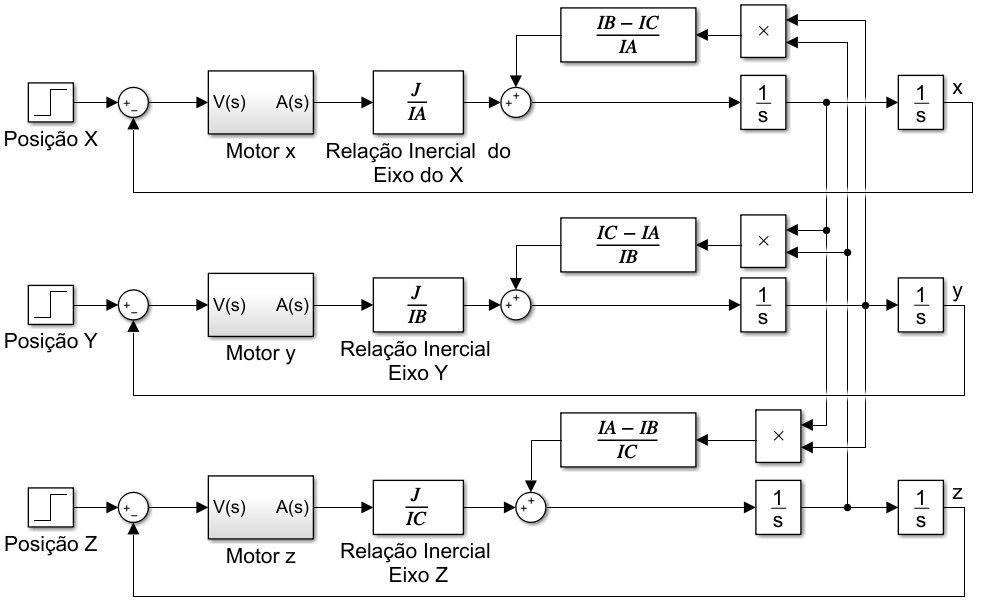
\includegraphics[scale=.6]{metodologia/img/simulink_modelo_completo_aberto}
  \end{center}
  \fonte{Elaborado pelo Autor.} 
  \label{fig:simulink_modelo_completo_aberto}
\end{figure}

Onde o bloco subsistema Motor x, y e z, é constituído pela função de transferência da equação \ref{eq:motor_accel}, que é inserida na ferramenta Matlab\copyright da seguinte forma:

\begin{figure}[H]
  \caption{Função de transferência dos motores.}
  \begin{center}
      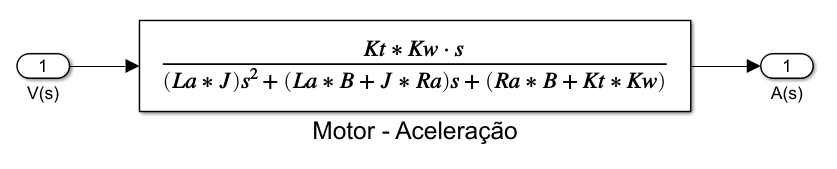
\includegraphics[scale=.6]{metodologia/img/modelo_satelite_motor}
  \end{center}
  \fonte{Elaborado pelo Autor.} 
  \label{fig:modelo_satelite_motor}
\end{figure}

Se fecharmos a malha em posição, usando um acelerômetro e usarmos um controlador PID, por consequência, conseguimos controlar a dinâmica do satélite em malha fechada. O diagrama de blocos com realimentação e com o controlador PID pode ser visto na figura \ref{fig:modelo_satelite_pid}. 

\begin{figure}[H]
  \caption{Modelo em malha fechada com um controlador PID.}
  \begin{center}
      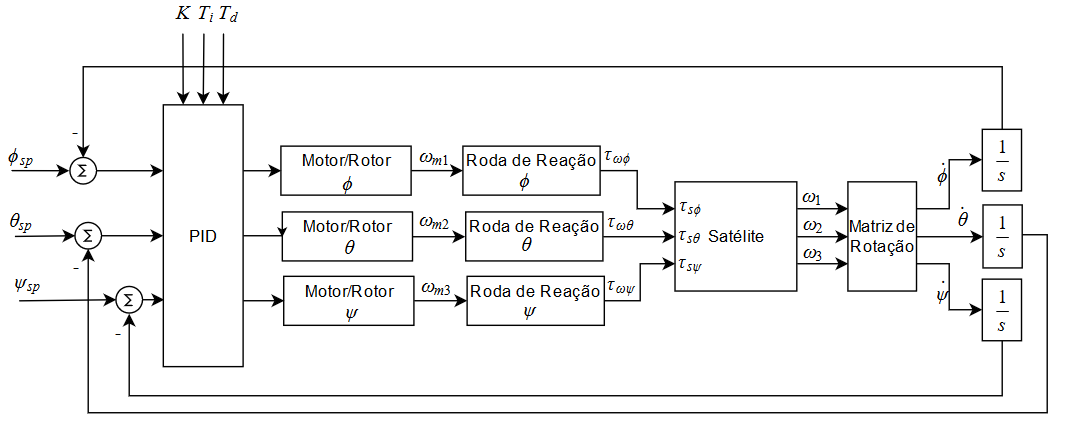
\includegraphics[scale=.6]{metodologia/img/modelo_satelite_pid}
  \end{center}
  \fonte{Elaborado pelo Autor.} 
  \label{fig:modelo_satelite_pid}
\end{figure}

Onde o bloco subsistema PID é constituído pelos seguintes blocos:

\begin{figure}[H]
  \caption{Digrama de blocos do controlador PID com Anti-Windup.}
  \begin{center}
      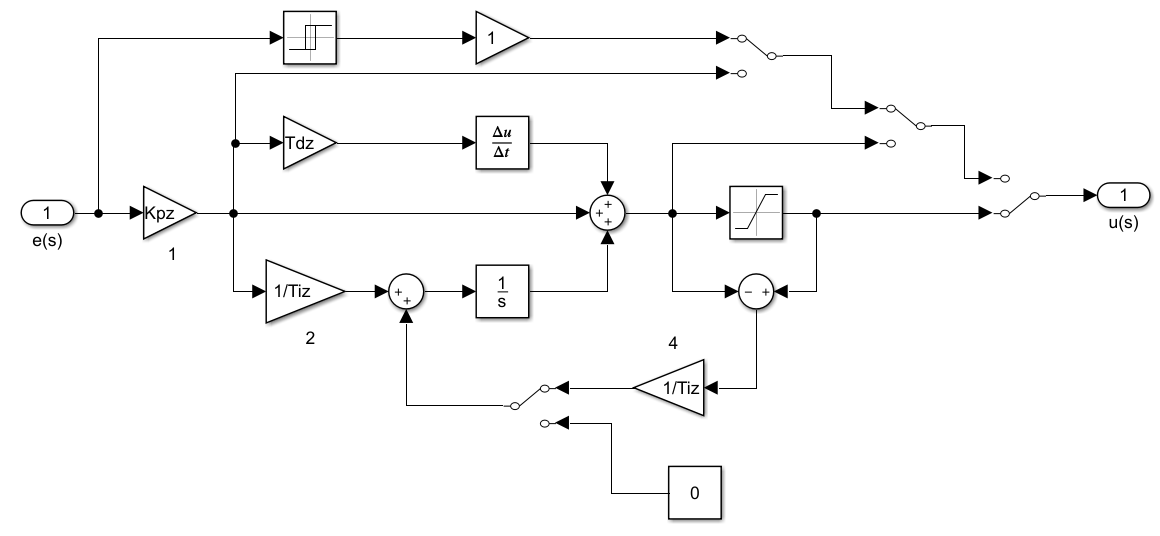
\includegraphics[scale=.55]{metodologia/img/matlab_pid_antiwindup}
  \end{center}
  \fonte{Elaborado pelo Autor.} 
  \label{fig:simulink_modelo_completo_aberto}
\end{figure}

Esse último diagrama é usado para o desenvolvimento do controle em \textit{software}, onde os parâmetros do controlador são estimados pelos diferentes tipos de sintonia descritos na revisão bibliográfica. Na sequência, serão descritos os métodos que serão utilizados para implementar esse modelo em Python e embarcar-lo na RPi.


%%%%%%%%%%%%%%%%%%%%%%%%%%%%%%%%%%%%%%%%%%%%%%%%%%%%%%%%%%%%%%%%%%%%%%

\section{\textit{Software}}

Após a modelagem, devemos implementar o modelo e configurar todas as interfaces com os atuadores e sistema supervisório. A figura \ref{fig:comunicacao_projeto} descreve a forma que se dá a comunicação entre os periféricos, através da interface I2C para a RPi se comunicar com o acelerômetro/giroscópio, PWMs (\textit{Pulse Width Modulation} - Modulação por Largura de Pulso) para a comunicação com os ESC e o protocolo SSH (\textit{Secure Shell}) para a comunicação com o usuário.

\begin{figure}[H]
  \caption{Representação geral do sistema.}
  \begin{center}
      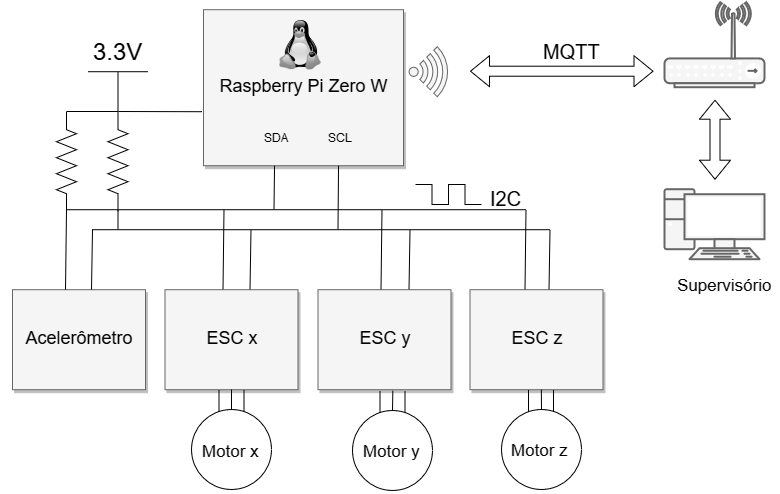
\includegraphics[scale=.75]{metodologia/img/comunicacao_projeto}
  \end{center}
  \fonte{Elaborado pelo Autor.} 
  \label{fig:comunicacao_projeto}
\end{figure}


Após modelada a topologia geral do sistema, é possível dividir a parte de \textit{software}, onde é descrita a implementação de cada etapa, começando com a implementação do controlador e da sua sintonia, que está na sequência.


%%%%%%%%%%%%%%%%%%%%%%%%%%%%%%%%%%%

\subsection{Implementação do Controlador PID e Métodos de Sintonia}

Nessa etapa, ocorre a implementação usando a linguagem de programação Python, a qual, possui diversas bibliotecas de controle, interfaceamento e protocolos de comunicação. O desenvolvimento foi orientado para o menor tempo possível de atualização das entradas e saídas, pois, como é uma linguagem \textit{script} sendo executada por um sistema operacional, algumas tarefas poderiam ser executadas em baixa prioridade, criando um comportamento não determinístico do período de amostragem. Uma solução para esse problema, foi a criação de uma interrupção via relógio que chama uma função de atualização das entradas e saídas, além do cálculo do PID e do filtro de Kalman. Na figura \ref{fig:software_model} podemos ver o fluxograma do \textit{script} de controle.

\begin{figure}[H]
  \caption{Fluxograma do \textit{software} de controle.}
  \begin{center}
      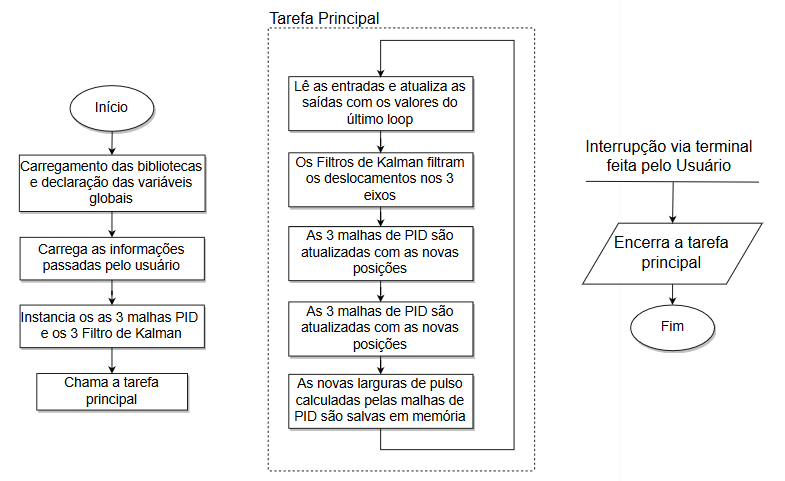
\includegraphics[scale=.65]{metodologia/img/software_model}
  \end{center}
  \fonte{Elaborado pelo Autor.} 
  \label{fig:software_model}
\end{figure}

Após o desenvolvimento das malhas de controle e testes preliminares, ficou clara a grande influência dos sinais provenientes do giroscópio no resultado final, necessitando uma análise minuciosa para possibilitar o perfeito funcionamento do filtro de Kalman e, por consequência, controlar o simulador de satélites. Isso é abordado na sequência. 


%%%%%%%%%%%%%%%%%%%%%%%%%%%%%%%%%%%

\subsection{Análise dos Sinais e Filtragem}

Ao fazer os primeiros testes, ficou perceptível o \textit{bias} (deslocamento em relação ao zero) e a gama de ruídos que compõem os sinais amostrados, isso pode ser visto na figura \ref{fig:bias_correction} (a), onde temos mais de 100.000 amostras nos três eixos. Já nas imagens \ref{fig:bias_correction} (b), (c) e (d), podemos ver o histograma dos mesmos sinais.

\begin{figure}[H]
  \caption{Características dos sinais amostrados pelo giroscópio.}
  %\begin{center}
      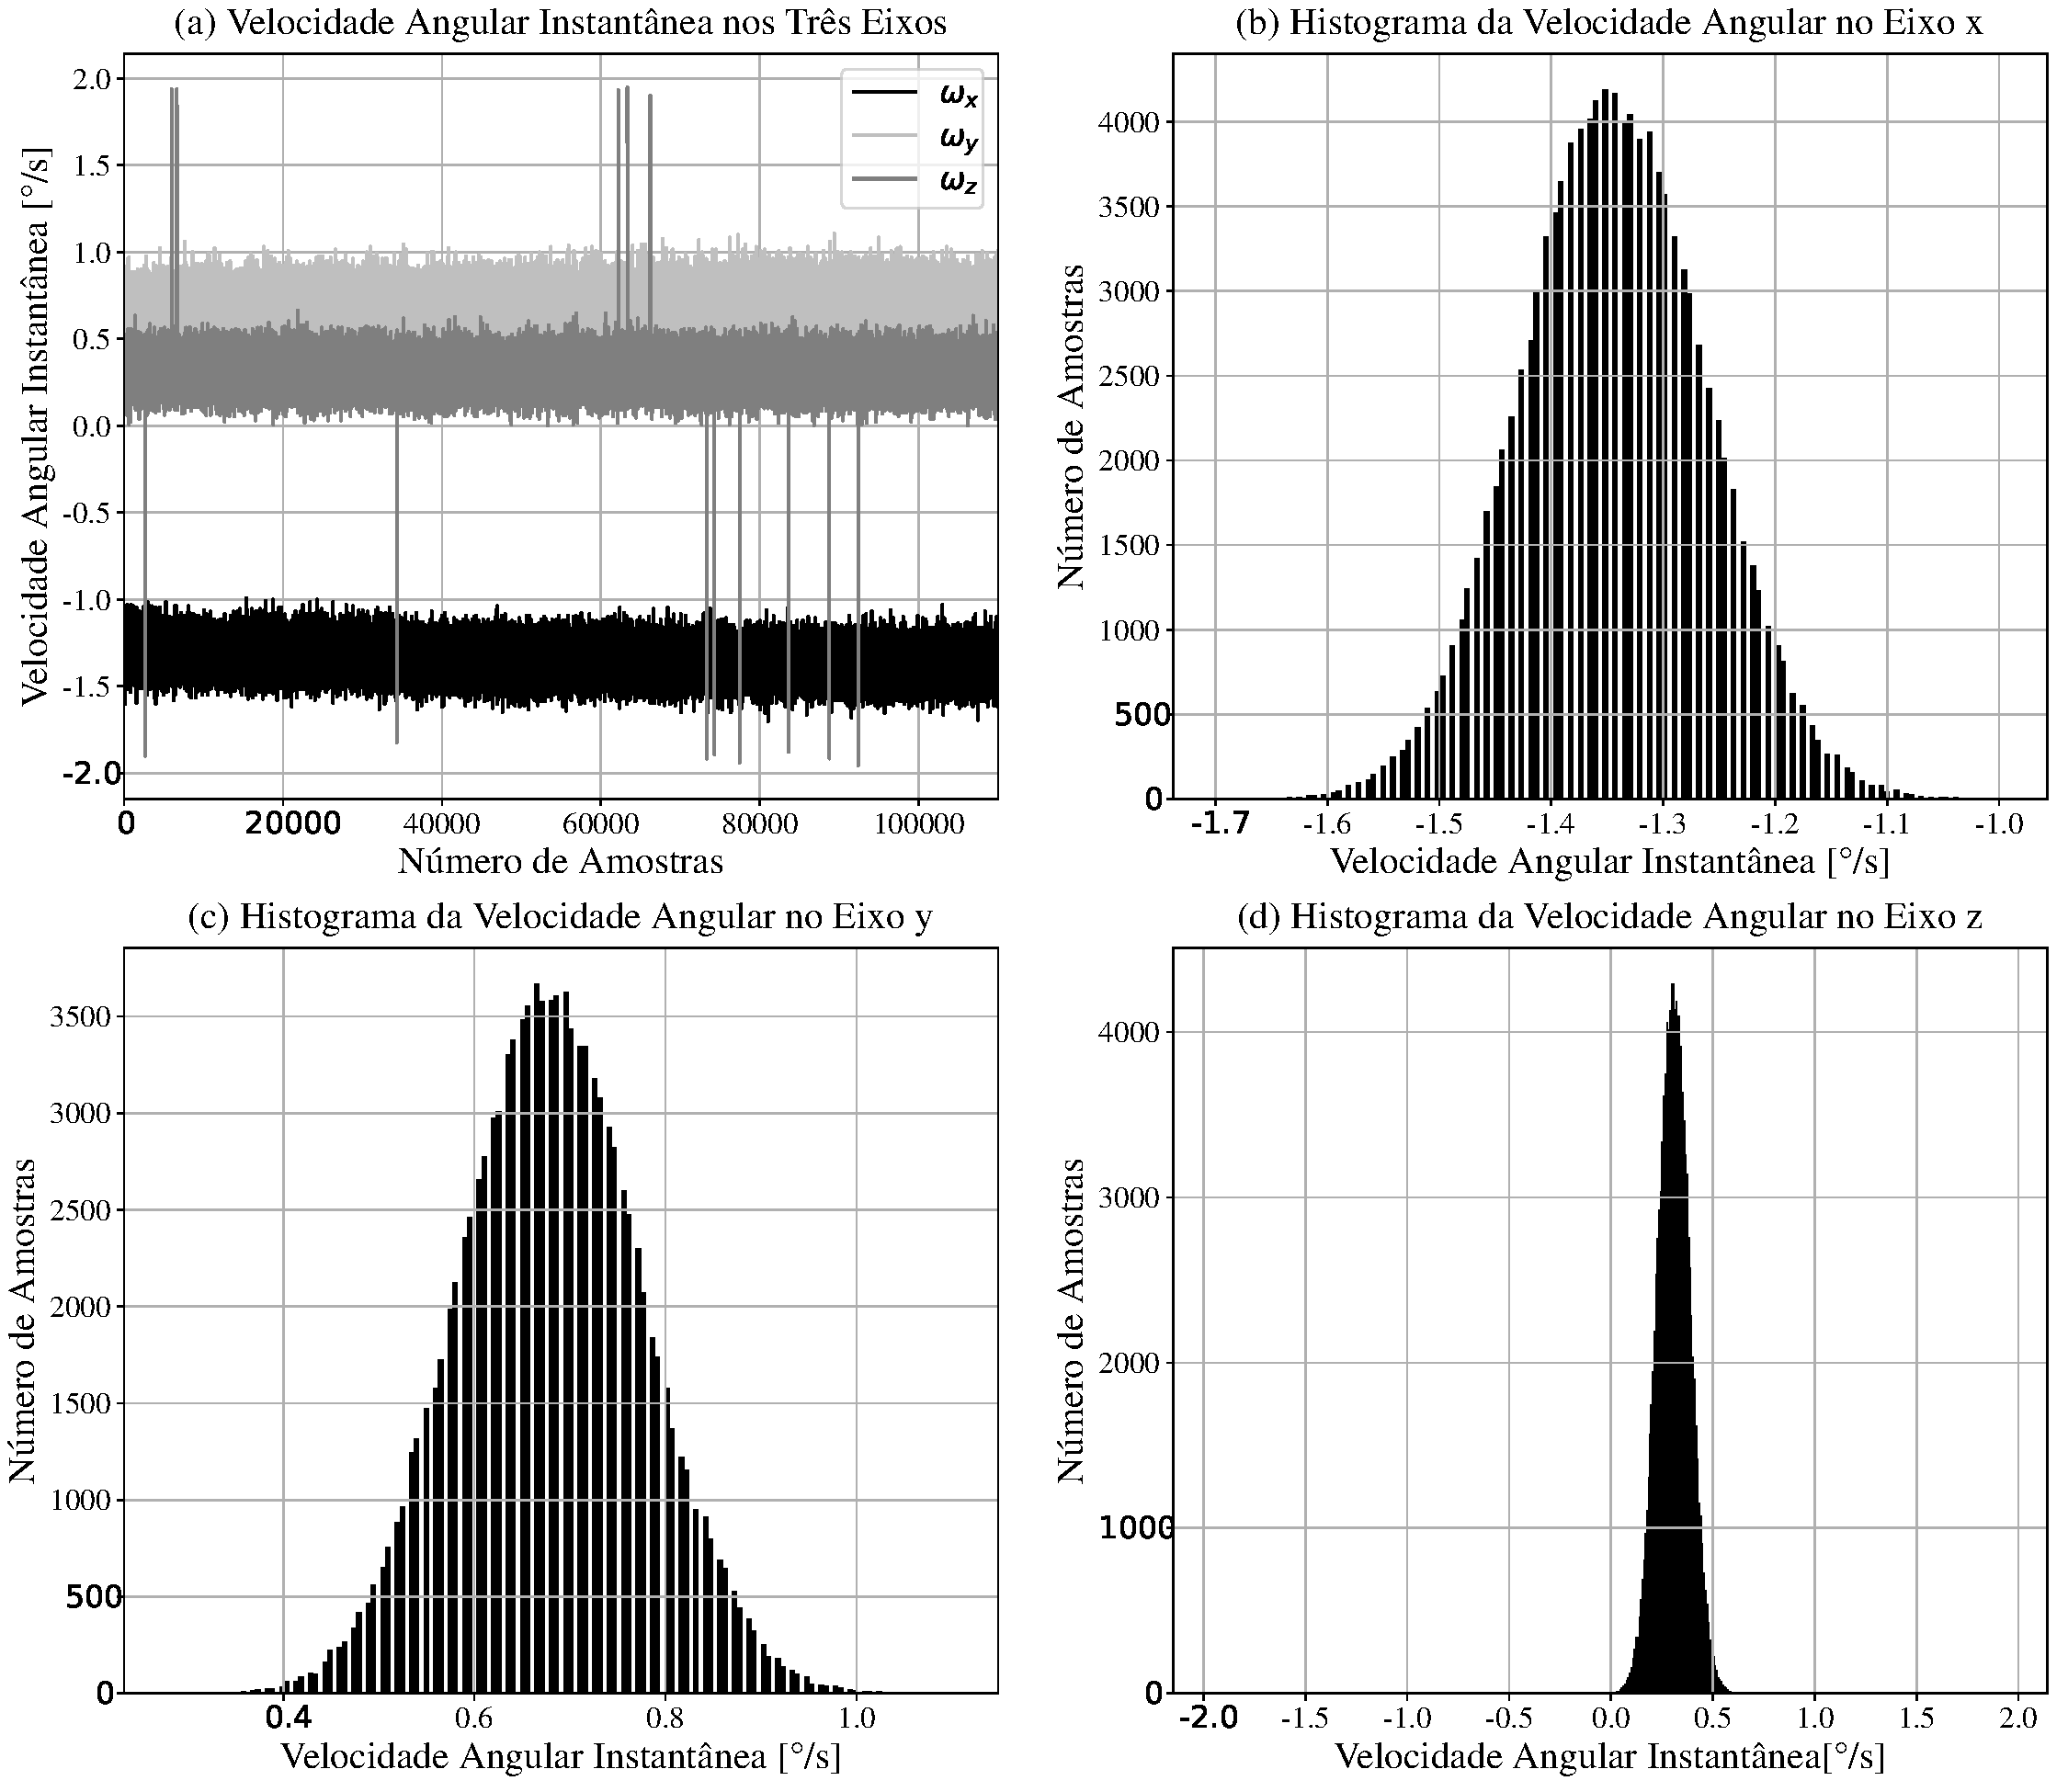
\includegraphics[scale=.4]{metodologia/img/bias_correction}
  %\end{center}
  \fonte{Elaborado pelo Autor.} 
  \label{fig:bias_correction}
\end{figure}

Como podemos ver, os três sinais possuem uma distribuição caraterística muito próxima de uma normal, mesmo que no eixo z exista ruídos espúrios maiores que nos demais eixos, o que valida o uso do Filtro de Kalman e a escolha da média aritmética das amostras como \textit{bias} para as amostras do giroscópio. Os valores calculados pode ser vistos na tabela \ref{tab:bias_correction} 

\begin{table}[H]
  \caption{Correção do \textit{bias} do giroscópio.}
  \label{tab:bias_correction}
  \centering%
  \begin{minipage}{.42\textwidth}
    \begin{tabular*}{\textwidth}{cc}
      \hline
      {Eixo} & Velocidade Angular ($\omega [\SI{}{\degree\per\second}]$)\\ \hline
      \hline
      x  &  -1.3441 \\ 
      y  &  0.6797 \\
      z  &  0.3071 \\ \hline
    \end{tabular*}
    \fonte{Elaborado pelo Autor.} 
  \end{minipage}
\end{table}

Essa etapa corrigiu os problemas enfrentados, o próximo passo é sintonizar as malhas de controle, isso é descrito na sequência.


%%%%%%%%%%%%%%%%%%%%%%%%%%%%%%%%%%%

\subsection{Métodos de Sintonia}

O último passo da implementação do satélite, é a sintonia das malhas de controle, onde diferentes métodos foram utilizados para descobrir os parâmetros \textit{$K_p$}, \textit{$K_i$} e \textit{$K_d$}. Para isso, usamos um método clássico de sintonia, que é o método do relé e por fim, o método automático usando redes neurais e regressão não-linear. Esses, serão descirtos na sequência. 


%%%%%%%%%%%%%%%%%%%%%%%%%%%%%%%%%%%

\subsubsection{Método do Relé}

A implementação desse método é simplesmente criarmos uma histerese sobre o erro, onde substituímos o sinal de controle por um valor fixo, fazendo o simulador de satélites oscilar ao tentar sair da região de histerese. Após a descoberta dos parâmetros que o levam  à oscilação sustentada, basta usarmos a equação \ref{eq:n(a)} e a tabela \ref{tab:Ziegler-Nichols-freq}.


%%%%%%%%%%%%%%%%%%%%%%%%%%%%%%%%%%%

\subsubsection{Método via RNA e Regressão Não-Linear}

Por fim, o método proposto pelo presente trabalho, onde diferentes conceitos foram empregados para a sintonia automática de controladores PID. Os dois usados, foram o de RNAs e regressão não-linear robusta, de onde são extraídos os novo valores dos parâmetros. Na figura \ref{fig:neural_regression} podemos ver a topologia usada.

\begin{figure}[H]
  \caption{Diagrama de blocos do sintonizador e otimizador.}
  \begin{center}
      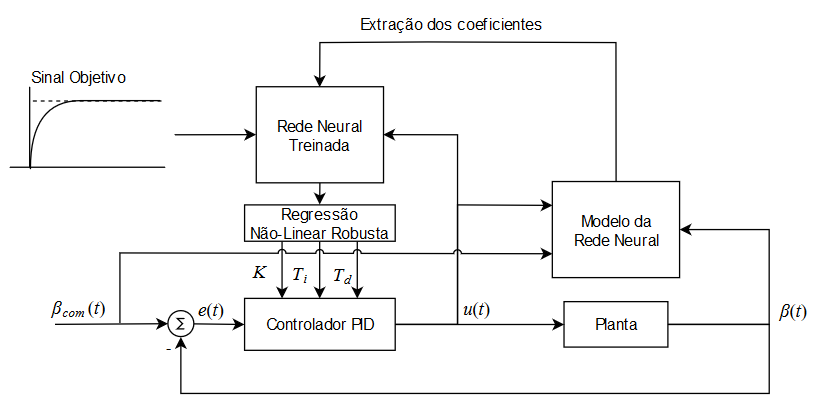
\includegraphics[scale=.65]{metodologia/img/neural_regression}
  \end{center}
  \fonte{Elaborado pelo Autor.} 
  \label{fig:neural_regression}
\end{figure}

O funcionamento dessa topologia é baseado na aprendizagem de máquina, onde uma RNA aprende o comportamento do satélite, tendo como entradas a posição atual ($\beta$) , o valor de referência ($\beta_{com}$) e o sinal de controle, que nada mais é do que a largura de pulso entregue ao motor. Temos como saída da RNA, o sinal de controle, pois esse na prática, é um sinal modulado contendo a largura de pulso para o motor, onde a rede neural é mais assertiva devido ao comportamento não-linear, também característico de uma RNA. Após o treinamento da RNA, ela é usada para se criar uma nova base de dados, onde ela recebe como parâmetros um sinal que é uma sugestão de resposta ao degrau (Sinal Objetivo) fornecida pelo usuário, ou ainda, uma representação do sistema em forma de um sistema de primeira ordem, pois esse, apresenta características melhores do que o sistema original. Basicamente, o objetivo de se fornecer esse sinal, é orientar a regressão não-linear ao ponto ótimo ou algo próximo a ele.

Por último, é feita e extração dos parâmetros do controlador via regressão, onde o antigo sinal de controle é modulado através da variação dos coeficientes do controlador PID discreto até possuir a forma de onda do novo sinal, que foi gerado pela rede neural. Essa regressão é feita usando como função de minimização, o próprio controlador PID discreto, como pode ser visto na equação da sequência:

\begin{equation}\label{eq:motor_accel}
u(t) = K_c e(t) + \frac{K_c}{T_i}\sum_{n=0}^{N}{e(t)dt}-K_cT_d\frac{P[n]-P[n-1]}{dt}
\end{equation}

Onde essa equação é análoga as equações do controlador PID discreto, descritas no referencial teórico, onde dt é a diferença de tempo entre as amostras, P é a variável de processo, e(t) é o erro instantâneo. A partir dessa equação, podemos implementar uma função de minimização, que está no código 1.

\begin{lstlisting}[caption={Minimização da função do controlador PID}]
funcao(Kp, Ti, Td, n, dados_objetivo, y_original, soma_erro) :
    erro = referencia - dados_objetivo[n]
    se (n>0) :
        soma_erro += erro
        derivada =  ({}dados_objetivo[n] -  dados_objetivo[n-1]/dt
        saida_controlador = Kp * erro + (Kp/Ti)*soma_erro*dt - Kp*Td*derivada
    se nao :
        saida_controlador = 0
    n += 1
    retorna saida_controlador - y_original
\end{lstlisting}

Onde \textit{n} é o indexador de cada interação, \textit{erro} é o erro no instante n, \textit{soma\_erro} é o somatório do erro, \textit{derivada} é a derivada da variável de interesse, \textit{dado\_teste} é o dado predito pela da RNA treinada, \textit{n} é o indexador das operações, \textit{saida\_controlador} é o sinal da saída do controlador, \textit{y\_original} é saída do controlador não sintonizado, \textit{dados\_objetivo} é o sinal da resposta objetivo, além dos já conhecidos parâmetros \textit{$K_p$, $T_i$ e $T_d$}. Com isso, conseguimos extrair os novos parâmetros do controlador.

%\chapter{Cronograma}

\begin{enumerate}
	\item \label{escolhatema} Estudo e escolha do tema.
	\item \label{refteorico} Fundamentação teórica.
	\item \label{metodologia} Estudo metodológico.
	\item \label{esctcci} Escrita do TCC I.
	\item \label{dimemecanica} Dimensionamento dos Elementos Mecânicos.
	\item \label{mecanica} Fabricação Mecânica do Satélite.
	\item \label{estudol} Estudo de Linux Embarcado e da Linguagem de Programação Python.
	\item \label{implementacao} Implementação dos Sistemas de controle em Python. 
	\item \label{integracaomec} Integração do Mecânica do Satélite com os Elementos Eletrônicos.
	\item \label{devapp} Desenvolvimento da camada de integração.
	\item \label{integracaosistema} Integração de todos os módulos que compõe o sistema.
	\item \label{testc} Testes e correções.
	\item \label{comapracoes} Comparar desempenho entre os diferentes tipos de Sintonia.
	\item \label{esctccii} Escrita do TCC II.
\end{enumerate}

\definecolor{midgray}{gray}{.5}
\begin{table}[!htbp]
	\centering
		\begin{tabular}{|c|c|c|c|c|c|c|c|c|c|c|}
		\hline
		&\multicolumn{9}{c|}{2018}\\
		\hline
		Fev.&Mar.&Abr.&Mai.&Jun.&Jul.&Ago.&Set.&Out.&Nov.\\
		\hline
		\ref{escolhatema}&\cellcolor{midgray}&&&&&&&&\\
		\hline
		\ref{refteorico}&&\cellcolor{midgray}&\cellcolor{midgray}&\cellcolor{midgray}&&&&&\\
		\hline
		\ref{metodologia}&&&\cellcolor{midgray}&\cellcolor{midgray}&&&&&\\
		\hline
		\ref{esctcci}&&\cellcolor{midgray}&\cellcolor{midgray}&\cellcolor{midgray}&&&&&\\
		\hline
		\ref{dimemecanica}&&&&&\cellcolor{midgray}&&&&\\
		\hline
		\ref{mecanica}&&&&&\cellcolor{midgray}&\cellcolor{midgray}&&&\\
		\hline	
		\ref{estudol}&&&&&&\cellcolor{midgray}&&&\\
		\hline
		\ref{implementacao}&&&&&&\cellcolor{midgray}&\cellcolor{midgray}&\cellcolor{midgray}&\\
		\hline
		\ref{integracaomec}&&&&&&&\cellcolor{midgray}&\cellcolor{midgray}&\\
		\hline
		\ref{devapp}&&&&&&&&\cellcolor{midgray}&\\
		\hline	
		\ref{integracaosistema}&&&&&&&&\cellcolor{midgray}&\\
		\hline	
		\ref{testc}&&&&&&&&\cellcolor{midgray}&\\
		\hline	
		\ref{comapracoes}&&&&&&&\cellcolor{midgray}&\cellcolor{midgray}&\cellcolor{midgray}\\
		\hline
		\ref{esctccii}&&&&&&&\cellcolor{midgray}&\cellcolor{midgray}&\cellcolor{midgray}\\
		\hline		
		\end{tabular}
\end{table}
\phantompart
% ||||||||||||||||||||||||||||||||||||||||||||||
% Capitulo de Resultados Preliminares
% ||||||||||||||||||||||||||||||||||||||||||||||

\chapter{Análise de Resultados}

Neste capítulo são apresentados os resultados do projeto, os quais são os produtos dos estudos de casos desenvolvidos nas empresas parceiras.
Como se trata de um estudo de caso, e para as empresas, uma prova de conceito, os resultados também foram divididos por equipamento avaliado:
exaustor e seleira universal. Os mesmo, inicialmente são apresentados capturas de telas do software na parte de análise dos sinais coletados, para fim
de dar uma visão global do estado de saúde do equipamento no dado momento. Na sequência, gráficos específicos, levantando características e 
comparações em diferentes condições, mostrando a relação de causa e efeito. Por fim, apontamentos e discussões sobre os resultados de cada um
dos elementos, e também comparações entre os mesmos.

Para a apresentação dos resultados do exaustor, foram feitas capturas de tela do software do sistema que estava instalado no motor, de forma
remota e supervisionada pelos responsáveis pela manutenção dos mesmos. A Figura \ref{fig:exaustor_1} é a captura de tela do sistema no dia
em que um relatório sobre a saúde dos exautores foi gerado, com os dados daquele momento, e com os limites gerados pelo ML
no momento da instalação (06/12/2020).

\begin{figure}[H]
    \caption{Captura de tela do sistema instalado no exaustor.}
    \begin{center}
        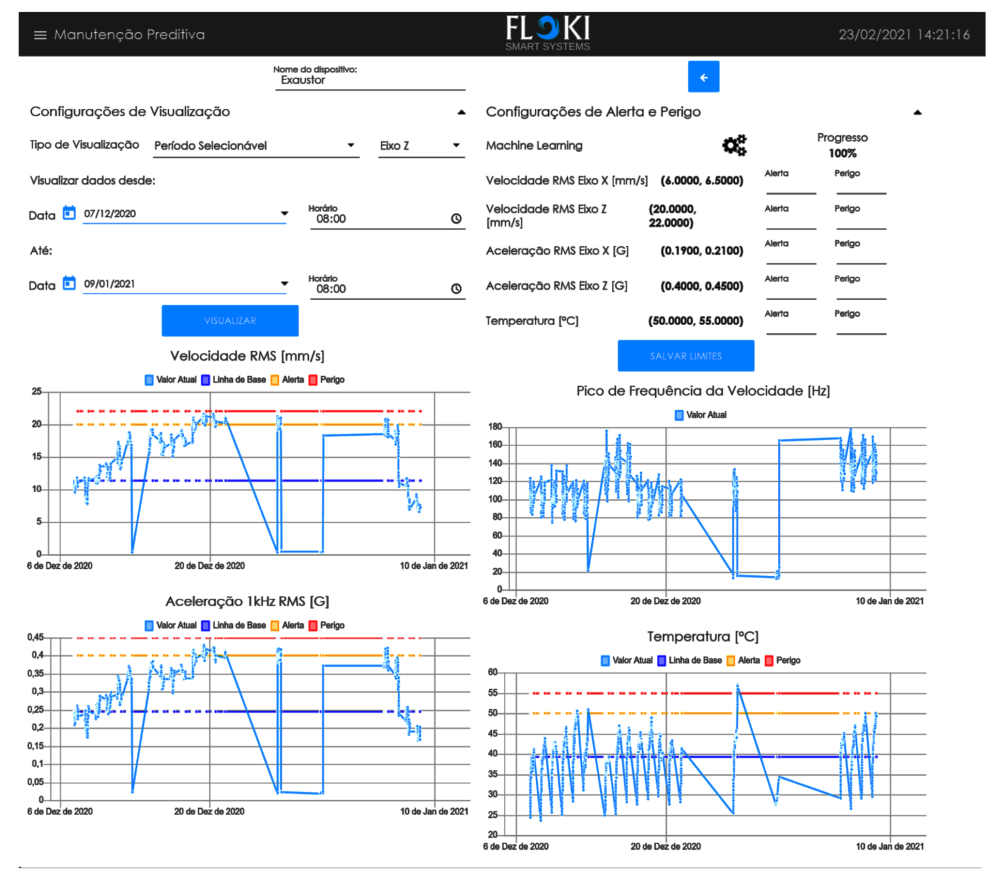
\includegraphics[scale=0.95, page=1]{resultados/img/resultados.pdf}
    \end{center}
    \fonte{Elaborado pelo Autor.} 
    \label{fig:exaustor_1}
\end{figure}

A captura de tela está com os dados de velocidade e aceleração do eixo Z, como podemos ver. Fica claro que as grandezas físicas
ultrapassam os limites estabelecidos pelo ML, somente no estado de alerta, mas isso não significa que o motor esteja em bom estado.
Se consultarmos a tabela \ref{tab:iso10816-1_randall_p146}, veremos que os valores para um motor de Classe II, segundo norma  ISO 10816-1, está 
entre apenas tolerável e não permitido, dependendo do regime de funcionamento. 
Se olharmos o eixo z, que se encontra na Figura \ref{fig:exaustor_xz}, os valores não permitidos, deixando claro o risco de falha iminente do 
motor.

\begin{figure}[H]
    \caption{Velocidade RMS [\SI{}{\milli\metre\per\second}] coletados do eixo x (A) e z (B).}
    \begin{center}
        \includegraphics[scale=0.65, page=2]{resultados/img/resultados.pdf}
    \end{center}
    \fonte{Elaborado pelo Autor.} 
    \label{fig:exaustor_xz}
\end{figure}

O eixo z se encontra em estado severo de vibração, não entrando em alarme devido ao ML tardio executado
pelo do operador, sendo agora uma tarefa de gestão do sistema, de se executar da maneira mais adequada, que é logo após o recondicionamento 
ou ajustar manualmente os limites de acordo com a norma ISO 10816-1. Outra característica importante é a temperatura, que pode ser vista na 
figura \ref{fig:exaustor_temperatura}, que teve uma dinâmica bem comportada e com característica de um sistema linear de primeira ordem.


\begin{figure}[H]
    \caption{Temperatura amostrada no exaustor.}
    \begin{center}
        \includegraphics[scale=0.65, page=3]{resultados/img/resultados.pdf}
    \end{center}
    \fonte{Elaborado pelo Autor.} 
    \label{fig:exaustor_temperatura}
\end{figure}

Fica nítido também o processo de aquecimento do dispositivo, seguindo os ciclos de funcionamento, que são bem regulares. O estudo de caso do 
exaustor se mostrou um ótimo caso para se analisar o comportamento do sistema em um dispositivo que já estava em funcionamento por um bom tempo 
após o recondicionamento, onde a técnica de ML, como esperado, não contribuiu com o objetivo de se detectar falhas, pois, as
condições iniciais não eram as ideais e os limites ficaram além dos permitidos. Mas o funcionamento geral da ferramenta foi excelente, sem nenhum
problema grave reportado, funcionando dentro das especificações e dentro do esperado pela empresa parceira. Um relatório foi gerado e entregue
para a empresa, contendo todos os dados e explicações, o qual foi aceito e sinalizaram o desejo de instalar em mais equipamentos.

A segunda prova de conceito foi realizada em uma seleira universal, como descrito anteriormente, onde 5 sensores foram distribuídos pela máquina, com o 
objetivo de monitorar os pontos críticos. Como no caso do exaustor, foram realizadas capturas de telas do sistema, onde a Figura
\ref{fig:seleira_universal} representa a captura dos dados do sensor 5, 4 dias antes de uma falha (08/12/2020). 

\begin{figure}[H]
    \caption{Linhas de base e sinais coletados em um dos 5 sensores na seleira universal.}
    \begin{center}
        \includegraphics[scale=0.9, page=4]{resultados/img/resultados.pdf}
    \end{center}
    \fonte{Elaborado pelo Autor.} 
    \label{fig:seleira_universal}
\end{figure}

Esta máquina não apresenta um processo contínuo como o exaustor, exigindo uma amostragem maior para se captar todas as características do 
funcionamento. Estes sensores foram instalados no dia 13/11/2020, mas os dados começaram a ser coletados apenas no dia 16/11/2020, onde a 
ferramenta de ML fui usada e os limites foram criados. 
A ferramenta foi aplicada em todos os 5 sensores, que foram instalados em acoplamentos, nas proximidades de polias e moto-redutores.
Cada um destes monitorou um comportamento diferente, mas o sensor mais importante se mostrou ser o 5, onde os resultados foram mais nítidos. 
Os outros sensores, pelo menos mais 3 apresentaram comportamento anômalos, mas nenhum como este. A Figura \ref{fig:seleira_universal_antes_depois}
apresenta uma comparação dos dados de velocidade logo após a instalação, com os dados na iminência de uma falha.

\begin{figure}[H]
    \caption{Linhas de base e dados de velocidade [\SI{}{\milli\metre\per\second} no momento da instalação
    (A) x próximo da falha (B).}
    \begin{center}
        \includegraphics[scale=0.65, page=5]{resultados/img/resultados.pdf}
    \end{center}
    \fonte{Elaborado pelo Autor.} 
    \label{fig:seleira_universal_antes_depois}
\end{figure}

Como podemos ver, os dados coletados na iminência da falha ultrapassam os limites de alerta e perigo, mesmo que não continuamente, mas
como a regra estabelecida na metodologia, da existência de 5 picos ou média acima dos limites, caracterizando uma alerta. Como são muitos dados,
um a cada $\SI{30}{\second}$, a visualização das retas de limites ficam comprometidas, e só é possível ver pela parte da tela onde se edita os
valores, ou pelos pontos azuis-escuros, amarelos e vermelhos no lado direito do gráfico. Além disso, é possível notar que no início do processo,
o sistema já se encontrava em uma situação pouco tolerável, segundo a norma ISO 10816-1, justificável por estarem instalados em partes que 
normalmente vibram mais, justamente por possuírem muitos elementos mecânicos e partes móveis. Por fim, a seleira universal apresentou o rompimento de uma
correia alguns dias após estes dados serem coletados e visualmente alertar uma condição severa de falha, consolidando o uso da ferramenta em
mais um equipamento, independente de ser um motor ou outro sistema mecânico. A aplicação funcionou perfeitamente, similar ao estudo de caso do
exaustor, apresentando apenas uma falha de salvar repetidas vezes os limites, que foi resolvida remotamente e incorporada ao software do projeto.
Uma peculiaridade de um sistema mancalizado, que difere de uma instalação em um motor elétrico de indução, é o comportamento da temperatura,
que pode ser visto na Figura \ref{fig:seleira_universal_temperatura}. 
Ela tem um perfil mais discreto, e não seguindo um sistema de primeira ordem, por não estar próximo de uma fonte de calor significativa, por isso
os limites gerados para algo com pouca variância, são limites muito próximos dos dados amostrados, ocorrendo falsos positivos apenas com a
variação da temperatura ambiente. A solução para isso, já prevista no início do projeto, é a possibilidade do operador alterar os limites, de 
acordo com a dinâmica que o sistema está inserido, não cabendo utilizar  ML onde há pouca variância ou o equipamento já se 
encontra em severo desgaste. 

\begin{figure}[H]
    \caption{Temperatura [\SI{}{\celsius}] amostrada na seleira universal.}
    \begin{center}
        \includegraphics[scale=0.8, page=6]{resultados/img/resultados.pdf}
    \end{center}
    \fonte{Elaborado pelo Autor.} 
    \label{fig:seleira_universal_temperatura}
\end{figure}

Após a escrita de todo o trabalho, indo desde o conhecimento mínimo para o entendimento das propostas, passando pela descrição dos métodos
empregados, até a análise dos resultados, foi possível ver o funcionamento satisfatório do projeto. O próximo capítulo apresenta as conclusões
gerais do projeto, com os trabalhos futuros.
% ----------------------------------------------
% CONCLUSÃO
% ----------------------------------------------
\chapter[Considerações Finais]{Considerações Finais}

A modelagem matemática rica e orientada à uma variável em comum, o torque, facilitou a modelagem, possibilitando a conexão de todos os modelos em um único, o que relaciona a tensão nos motores com a posição do satélite. 

Após a modelagem completa do simulador de satélite, desde o projeto mecânico, controle e software e assimilando essas etapas com o cronograma, o projeto se mostra implementável em tempo hábil. Algumas etapas podem sofrer escorregamento, estendendo o tempo estimado, principalmente as etapas da implementação do sistema de controle em Python e a fabricação mecânica. Essa última é crítica, pois são necessários equipamentos com precisão e existe o risco de não conformidade das peças, criando retrabalhos. Ainda, todos os materiais são de fácil aquisição e desenvolvimento.


% ==============================================
% ELEMENTOS PÓS-TEXTUAIS
% ==============================================
\postextual
% ==============================================
% Referências bibliográficas
% ==============================================
\bibliography{referencial/references}
% ==============================================
% Glossário
% ==============================================
\glossary
% ||||||||||||||||||||||||||||||||||||||||||||||
% Apêndices
% ||||||||||||||||||||||||||||||||||||||||||||||
\begin{apendicesenv}
\partapendices
% ----------------------------------------------
% Apêndice 1
% ----------------------------------------------
\chapter{Código em C}
  \begin{lstlisting}
    #include <stdio.h>

    void main(void)
    {
    	return 0;
    }
  \end{lstlisting}
\end{apendicesenv}
% ||||||||||||||||||||||||||||||||||||||||||||||
% ANEXOS
% ||||||||||||||||||||||||||||||||||||||||||||||
%\begin{anexosenv}
\partanexos
% ----------------------------------------------
% Anexo 1
% ----------------------------------------------
\chapter{Datasheet}\label{anexo1}
%\includepdf[pages=-]{pdfs/Datasheet.pdf}%
\end{anexosenv}
% ==============================================
% INDICE REMISSIVO
% ==============================================
%\phantompart
%\printindex
% ----------------------------------------------

\end{document}